% Banking Management System - project report % Compile with: pdflatex report.tex (twice)
\documentclass[11pt,a4paper]{article}

\usepackage[T1]{fontenc}
\usepackage[utf8]{inputenc}
\usepackage{lmodern}
\usepackage[margin=0.6in]{geometry}
\usepackage{xcolor}
\usepackage{listings}
\usepackage{graphicx}
\usepackage{float}
\usepackage{longtable}
\usepackage{array}
\usepackage{parskip}
\usepackage{enumitem}
\usepackage{hyperref}
\hypersetup{hidelinks}
\graphicspath{{docs/}{docs/screenshots/}{../docs/}{../docs/screenshots/}}

\definecolor{codebg}{RGB}{248,248,248}
\definecolor{codekw}{RGB}{0,0,180}
\definecolor{codestr}{RGB}{0,120,0}
\definecolor{codecom}{RGB}{120,120,120}

\lstdefinestyle{c}{
language=C, basicstyle=\ttfamily\small, keywordstyle=\color{codekw}\bfseries, commentstyle=\color{codecom}\itshape, stringstyle=\color{codestr}, backgroundcolor=\color{codebg}, showstringspaces=false, breaklines=true, columns=fullflexible, keepspaces=true, frame=single, rulecolor=\color{gray!40}, framexleftmargin=4pt, xleftmargin=8pt, aboveskip=10pt, belowskip=10pt }

\lstdefinestyle{term}{
basicstyle=\ttfamily\footnotesize, backgroundcolor=\color{codebg}, breaklines=true, columns=fullflexible, keepspaces=true, frame=single, rulecolor=\color{gray!40}, framexleftmargin=4pt, xleftmargin=8pt, aboveskip=10pt, belowskip=10pt }

\newcolumntype{L}[1]{>{\raggedright\arraybackslash}p{#1}}

\setlist[itemize]{itemsep=2pt,topsep=3pt,parsep=0pt,partopsep=0pt}
\setlist[enumerate]{itemsep=2pt,topsep=3pt,parsep=0pt,partopsep=0pt}

\title{Banking Management System}
\author{Aradhya Chakrabarti (MT2026012)}
\date{CS-513 System Software Mini Project\\ International Institute of Information Technology, Bangalore}

\begin{document}
\raggedbottom
\setlength{\emergencystretch}{3em}
\maketitle

\section{Functional design}
\label{sec:fdd}

\subsection{Purpose and scope}

We need to design a banking management system which works over a command line interface. A separate server process should store its data on the filesystem and serve multiple clients over localhost. The client should provide a menu-based interface to the user. The server should be able to process requests from different kinds of users and show the relevant menu items for each role.

\subsection{Actors}

\begin{longtable}{L{0.22\linewidth}L{0.70\linewidth}}
\hline
Actor & Responsibility \\
\hline
Customer & Manages a personal account, transfers funds, applies for a loan, changes the password, views history, and gives feedback. \\
Employee & Opens and maintains customer accounts, views passbooks, closes eligible accounts, and decides assigned loans. \\
Manager & Activates or deactivates customers, assigns pending loans, and reviews feedback. \\
Administrator & Manages staff, user roles, user details, and the audit trail. \\
System & Handles sessions, permissions, locking, atomic commits, durability, and audit logging. \\
\hline
\end{longtable}

\subsection{Functional requirements}

\begin{longtable}{L{0.14\linewidth}L{0.78\linewidth}}
\hline
S.No. & Requirement \\
\hline
\endhead
\hline
\multicolumn{2}{l}{\textit{Authentication and sessions}} \\
\hline
AUTH-01 & A user logs in with a username and password. \\
AUTH-02 & Passwords are stored as salted hashes, never as clear text. \\
AUTH-03 & A user has at most one active session. \\
AUTH-04 & A deactivated or closed account cannot log in. \\
AUTH-05 & A user can change the password after proving the old one. \\
AUTH-06 & Logout ends the session and keeps the client open. \\
AUTH-07 & Exit logs out first and closes the client. \\
AUTH-08 & A role change or account deactivation revokes the live session. \\
\hline
\multicolumn{2}{l}{\textit{Customer operations}} \\
\hline
CUST-01 & The customer can view the current balance. \\
CUST-02 & A deposit increases the balance and writes one ledger row. \\
CUST-03 & A withdrawal decreases the balance and cannot overdraw it. \\
CUST-04 & A transfer debits the sender and credits the recipient in one atomic change. \\
CUST-05 & A customer can apply for a loan with an amount, a term, and a purpose. \\
CUST-06 & The customer can view a passbook of their own transactions. \\
CUST-07 & A transfer appears once for the sender and once for the recipient. \\
CUST-08 & The customer can submit feedback. \\
CUST-09 & The customer can read manager replies to their feedback. \\
CUST-10 & The customer can view a mini statement. \\
CUST-11 & Customer operations are refused for other roles. \\
\hline
\multicolumn{2}{l}{\textit{Employee operations}} \\
\hline
EMP-01 & An employee can add a customer with a unique username and an opening balance. \\
EMP-02 & A duplicate username is rejected. \\
EMP-03 & An employee can change a customer's name or reset the customer password. \\
EMP-04 & The employee can view a customer's passbook. \\
EMP-05 & The employee can list only the loans assigned to them. \\
EMP-06 & The employee can approve or reject an assigned pending loan. \\
EMP-07 & An employee cannot decide a loan assigned to another employee. \\
EMP-08 & An employee can close a customer account with a zero balance and no outstanding loan. \\
EMP-09 & The employee can change their own password. \\
\hline
\multicolumn{2}{l}{\textit{Manager operations}} \\
\hline
MGR-01 & A manager can activate or deactivate a customer account. \\
MGR-02 & A manager can assign a pending loan to an active employee. \\
MGR-03 & A manager can list pending loans. \\
MGR-04 & A manager can list feedback and mark it reviewed with a reply. \\
MGR-05 & The manager can change their own password. \\
\hline
\multicolumn{2}{l}{\textit{Administrator operations}} \\
\hline
ADM-01 & An administrator can add an employee or a manager. \\
ADM-02 & An administrator can modify any user's name or password. \\
ADM-03 & An administrator can change a user's role among customer, employee, manager, and administrator. \\
ADM-04 & An administrator cannot change their own role. \\
ADM-05 & An administrator can list all users. \\
ADM-06 & An administrator can read the audit trail. \\
ADM-07 & The administrator can change their own password. \\
ADM-08 & An administrator can set the single bank-wide loan interest rate and method. Existing loans keep the policy copied when they were created. \\
\hline
\multicolumn{2}{l}{\textit{System requirements}} \\
\hline
SYS-01 & The server serves multiple clients concurrently. \\
SYS-02 & Conflicting reads and writes are serialized. \\
SYS-03 & A multi-record operation commits atomically. \\
SYS-04 & A committed transaction survives a crash. \\
SYS-05 & An uncommitted transaction is not applied. \\
SYS-06 & State-changing operations are audited. \\
SYS-07 & Shutdown stops children, closes IPC objects, and releases the data lock. \\
SYS-08 & A handler does not outlive a crashed server parent. \\
SYS-09 & Only one server process should use a data directory at a time. \\
\hline
\end{longtable}

\subsection{Business rules}

\paragraph{Money.}
\begin{itemize}
\item The system should store every amount as an integer number of paise, where one rupee is 100 paise. This keeps INR amounts exact to two decimal places.
\item The system should accept only positive deposit and withdrawal amounts. A balance should never become negative.
\item A transfer should debit and credit the same amount. It should reject a transfer to the same account and a recipient who is not an active customer.
\item When an employee approves a loan, the system should credit the principal to the customer's balance once. A rejected loan should leave the balance unchanged.
\item An account should close only when the balance is zero and there is no pending or approved loan.
\end{itemize}

\paragraph{Accounts and roles.}
\begin{itemize}
\item Usernames should be unique and case-sensitive. Each user should have one role.
\item An administrator should not change their own role.
\item Only active accounts should be able to log in and move money.
\item A role or status change should end the target user's live session.
\item A closed account should keep its username and history, and the username should not be reused.
\end{itemize}

\paragraph{Loans.}
\begin{itemize}
\item A loan should move through three states: pending, approved, and rejected. Only a customer should apply.
\item The amount and term should be positive. The purpose should be stored with the application.
\item The administrator should set one annual interest rate and one method, simple or compound. The initial rate should be 0.00\% and the initial method should be simple.
\item When a customer applies, the application should copy the current policy into the loan and store the interest and total payable.
\item A later policy change should affect only new loans. Existing pending and approved loans should keep the policy they were created with.
\item Only a pending loan should be assigned or decided.
\item Approval should credit the principal and write a loan transaction. Rejection should change only the status.
\end{itemize}

\paragraph{Feedback.}
\begin{itemize}
\item Only a customer should submit feedback.
\item A new feedback record should have the status new.
\item A manager should mark it reviewed and write a reply.
\item The customer should be able to read the reply.
\end{itemize}

\paragraph{Sessions and audit.}
\begin{itemize}
\item Each session should belong to one user and one handler process.
\item The server should check the session table for every authenticated request.
\item Deactivation, account closure, role change, and logout should remove the session.
\item Every state-changing operation should post an audit record. The logger thread should write a timestamped line to the audit file.
\end{itemize}

\subsection{Data requirements}

\begin{longtable}{L{0.20\linewidth}L{0.18\linewidth}L{0.54\linewidth}}
\hline
Entity & Key & Fields \\
\hline
\endhead
User & id & username, name, role, active flag, salt, password hash, balance, created time \\
Loan & id & customer id, employee id, principal, term, status, interest method, rate, interest amount, total payable, purpose, applied and decided times \\
Transaction & id & user id, type, amount, balance after, timestamp, note \\
Feedback & id & user id, status, timestamp, message, reply \\
Session & slot & user id, handler pid, active flag \\
Audit entry & position & timestamp, user id, action text \\
\hline
\end{longtable}

A customer can have loans, transactions, and feedback. Employees process loans. Managers assign loans, change customer status, and review feedback. A user can have at most one session. An audit entry should name the user who performed the action.

\subsection{Personas}

We need to support four roles: customer, employee, manager, and administrator. Figure~\ref{fig:personas} shows their main actions and the interactions between them. The client menus follow these roles.

\begin{figure}[H]
  \centering
  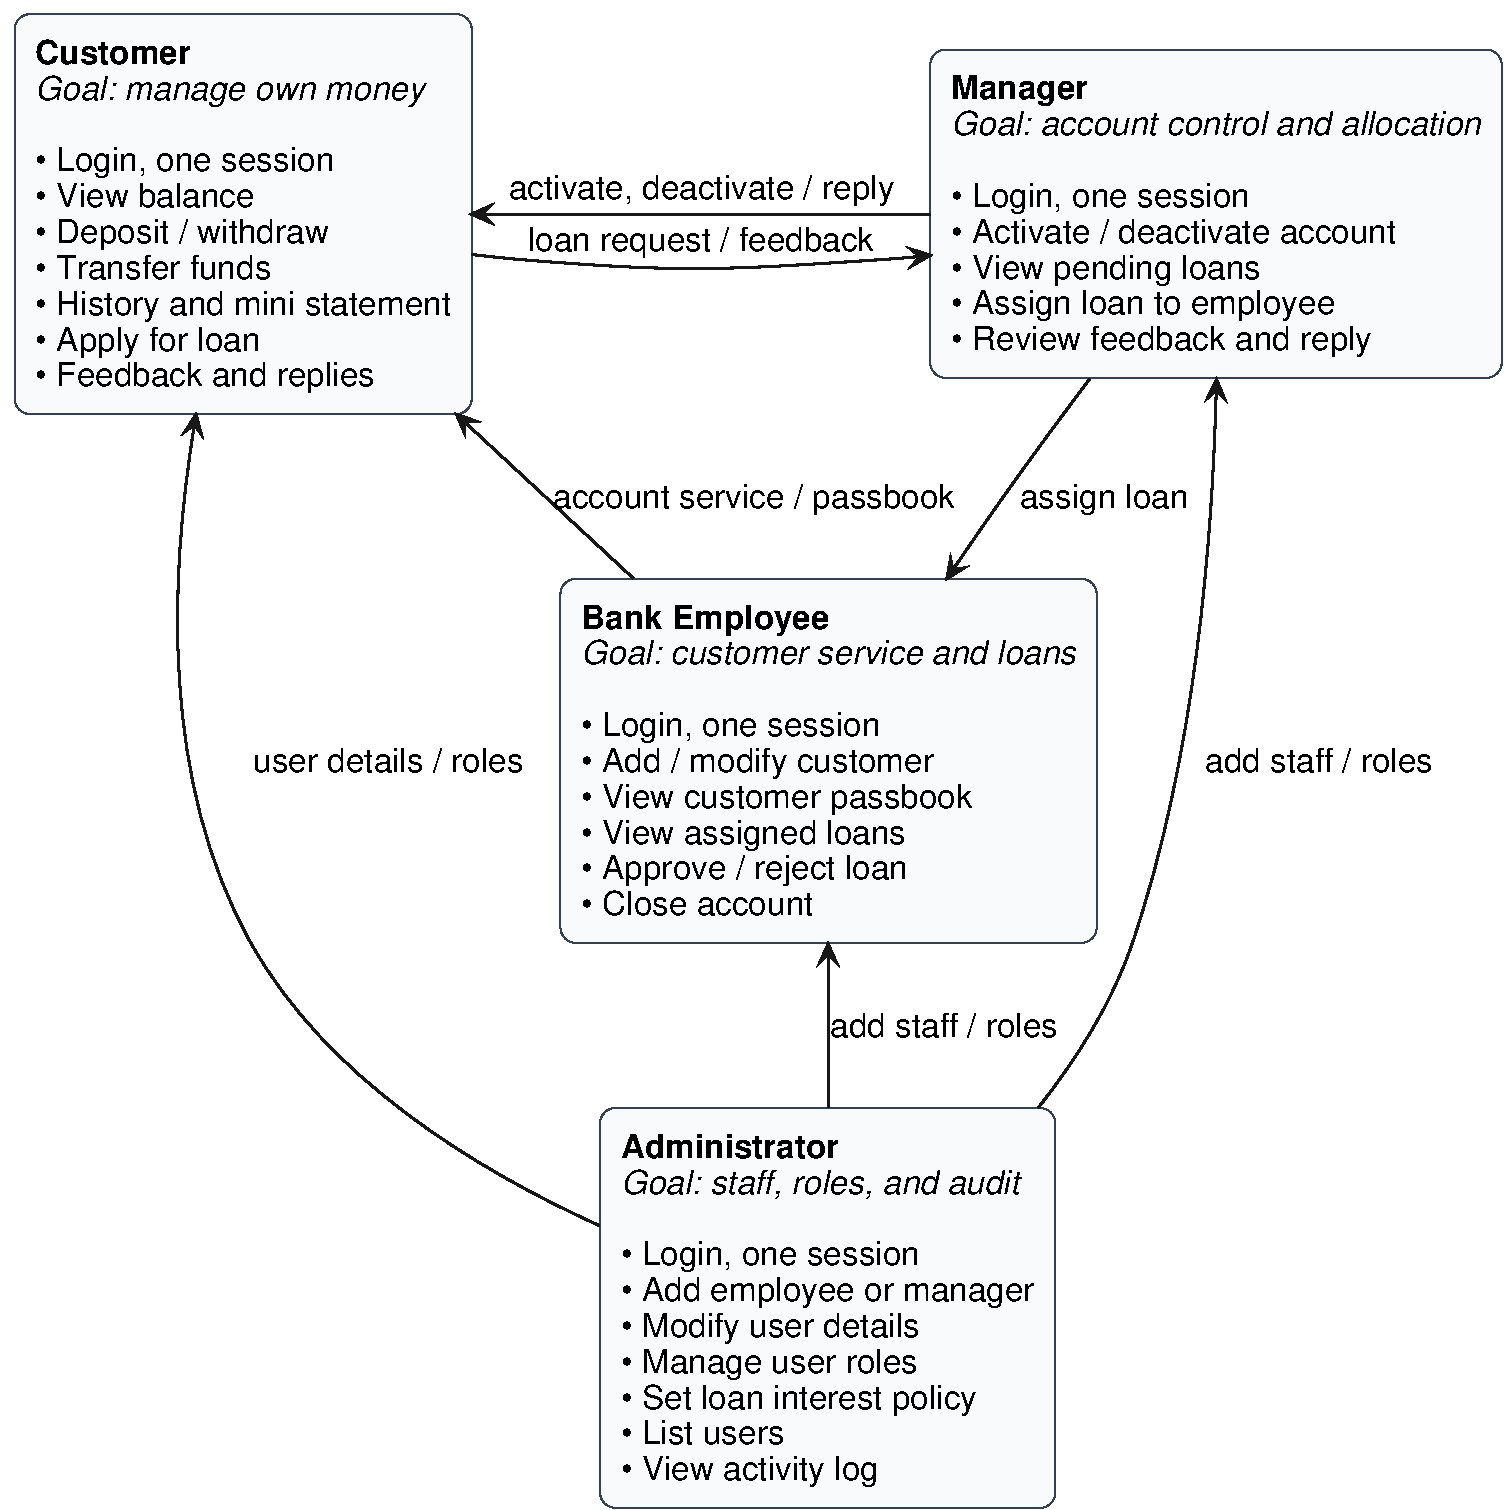
\includegraphics[width=0.88\linewidth]{personas_cards.pdf}
\caption{Role personas, their main actions, and the main interactions.}
  \label{fig:personas}
\end{figure}

\subsection{Non-functional requirements}

\begin{itemize}
\item Concurrency: several clients should be able to work at the same time. Readers should take shared record locks, and writers should take one whole-file lock.
\item Atomicity: a multi-record operation should write the complete new database or leave the previous database untouched.
\item Consistency: business checks should run while the writer holds the database lock.
\item Isolation: a reader should not read a record while a writer holds the whole-file lock, and it should not see the temporary file.
\item Durability: the temporary file and the directory should be flushed before the server reports success.
\item Capacity: the design should support 200 users, 200 loans, 2000 transactions, 200 feedback records, and 64 sessions.
\item Security: the server should store salted password hashes, check roles and sessions, keep data files at mode 0600, and write an audit trail.
\item Portability: the implementation should use C17 and POSIX/Linux system calls with plain files.
\item Visibility: the server should print startup messages and write a timestamped audit file.
\end{itemize}

\section{Technical design}
\label{sec:tdd}

\subsection{System Design}

We need two programs. The server process should use the data directory for storage, create the System V IPC objects, and listen on the socket. The client should connect to \texttt{127.0.0.1:9099} by default and show the role menus.

The server parent should accept a connection and fork one handler child for the whole client session. The parent should use \texttt{select} on the listening socket and a self-pipe for signals. The child should use \texttt{select} with a one-second timeout so that it can notice a shutdown even when the client is quiet. A logger thread in the parent should read audit events from the message queue.

Figure~\ref{fig:architecture} shows the system components and design.

\begin{figure}[H]
  \centering
  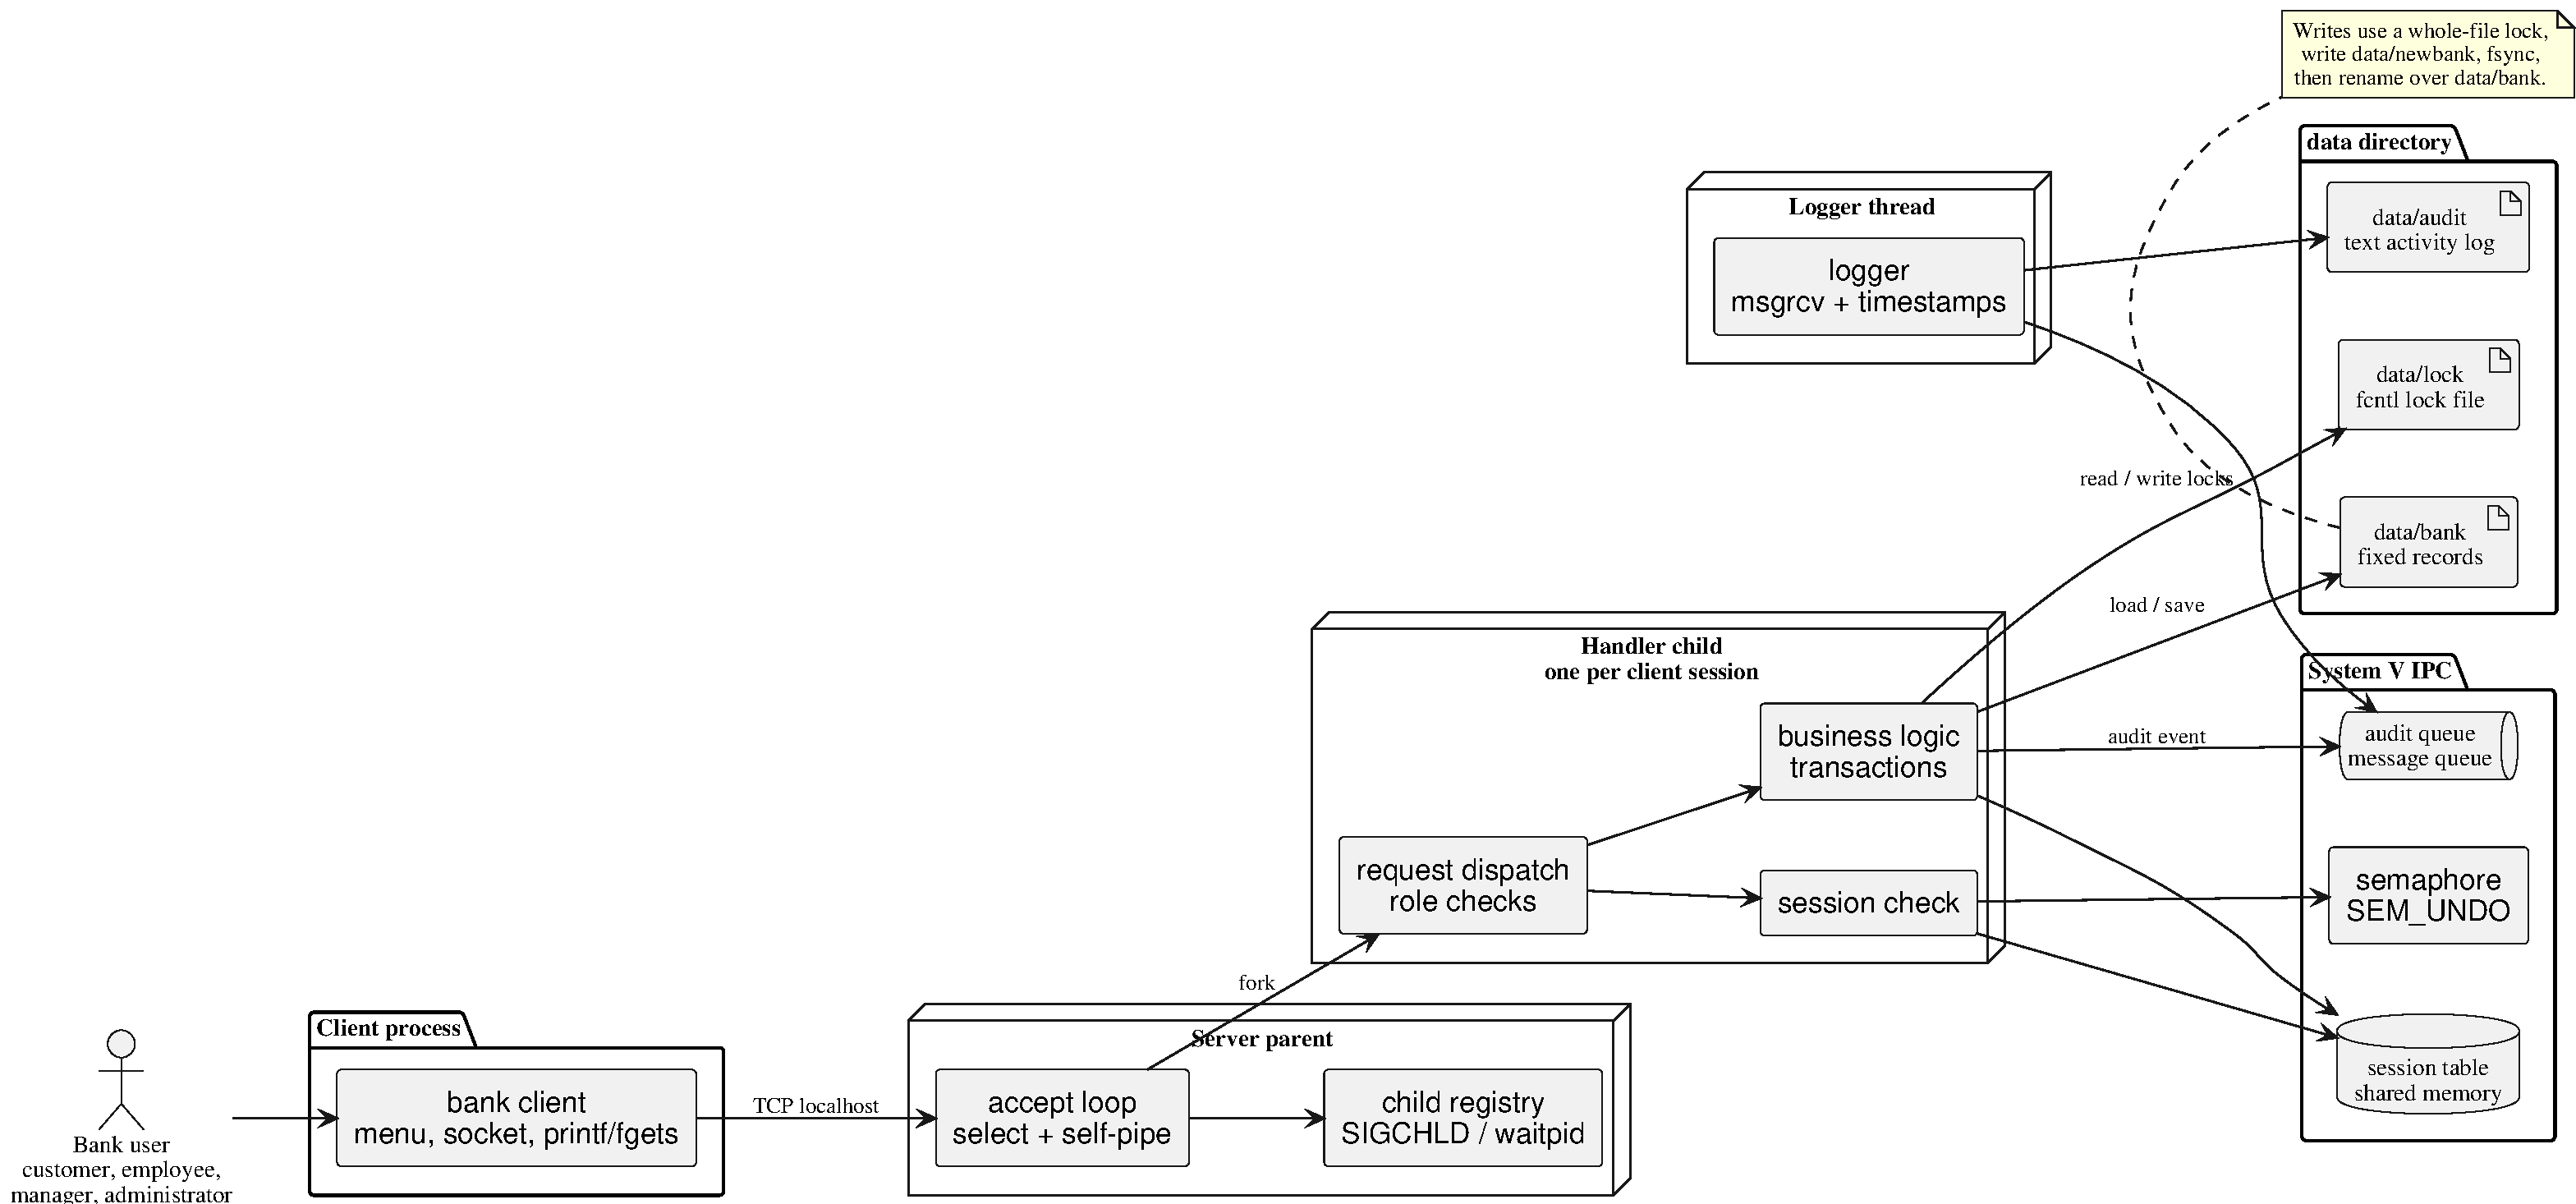
\includegraphics[width=0.98\linewidth]{architecture.pdf}
\caption{System components and design.}
  \label{fig:architecture}
\end{figure}

\subsection{Storage design}

We need to keep all persistent state in one binary file, \texttt{data/bank}. The file should contain a header and fixed-size arrays for users, loans, transactions, and feedback. The data files are extensionless.

\begin{longtable}{L{0.16\linewidth}L{0.70\linewidth}}
\hline
Region & Contents \\
\hline
Header & File identifier, next ids, row counts, bank-wide loan rate and method. \\
\texttt{users[]} & Username, display name, salted hash, role, active flag, balance, creation time. \\
\texttt{loans[]} & Customer and employee ids, principal, term, status, rate and method snapshot, interest, total payable, purpose, timestamps. \\
\texttt{txns[]} & User id, type, amount, balance after, timestamp, note. \\
\texttt{feedback[]} & User id, status, timestamp, message, manager reply. \\
\hline
\end{longtable}

The header should store a file identifier, the next id for each table, and the number of used rows. A user record should store the role, active flag, username, display name, salt, password hash, balance, and timestamps. The balance is part of the user record, so one row represents a customer account. A transaction record should store the user id, type, amount, balance after the movement, time, and note. A transfer should create two rows, one for each party.

\begin{longtable}{L{0.16\linewidth}L{0.22\linewidth}L{0.50\linewidth}}
\hline
File & Purpose & Format \\
\hline
\texttt{data/bank} & Complete database & Binary \texttt{struct bank} \\
\texttt{data/newbank} & Staging file for a commit & Same binary layout \\
\texttt{data/lock} & Lock target & Empty file used only by \texttt{fcntl} \\
\texttt{data/audit} & Activity log & Timestamped text lines \\
\hline
\end{longtable}

The server should write the complete staging file, flush it, and rename it over \texttt{data/bank}. We should keep the lock file separate, so a rename does not affect locks.

\subsection{Runtime design}

\begin{itemize}
\item Read locks: a reader should take a shared \texttt{fcntl} lock on the byte range for the record in \texttt{data/lock}, read the record from \texttt{data/bank}, and release the lock. Reads lock the separate lock file because a writer replaces \texttt{data/bank}.
\item Write locks and commit: a writer should take an exclusive lock on the whole \texttt{data/lock} file, load the database, run the business checks, and change the copy in memory. It should write the complete image to \texttt{data/newbank}, call \texttt{fsync}, rename it over \texttt{data/bank}, call \texttt{fsync} on the directory, and release the lock. The rename leaves either the old complete file or the new complete file, so a crash cannot leave a half-written database and a journal is unnecessary. The database is small, so one whole-file lock is simpler than a record-level write transaction.
\item Sessions: the server uses System V shared memory to store the session table, and one semaphore protects it. Login should add one slot per user, every request should check the slot, and logout, deactivation, account closure, role change, or child exit should remove it.
\item Processes and signals: the parent should accept connections and fork one handler child per client. It should use \texttt{select} on the listening socket and the read end of a self-pipe. Handlers for \texttt{SIGCHLD}, \texttt{SIGTERM}, and \texttt{SIGINT} should write one byte, so the parent does the work after \texttt{select} returns. The parent should read the pipe, collect exited children with \texttt{waitpid(-1, NULL, WNOHANG)}, and remove their sessions. The child should ignore \texttt{SIGPIPE} and exit if its parent changes because the server is gone.
\item Requests and audit: the client and server should exchange fixed-size request and response values. The dispatcher should handle login separately and should check the session, active flag, and role for every other operation. Handlers should use \texttt{begin\_write} or the read helpers, and successful writes should post an audit event to the message queue, where one logger thread writes it.
\end{itemize}

\subsection{Security}

The server should store passwords as a per-user salt and a 64-bit FNV-1a hash. The salt comes from the current time and process id. To verify a password, the server recomputes the hash and compares the result.

The server should create data files with mode 0600 inside a directory with mode 0700. It should check the active flag, the session table, and the role on every request. The client and server should use plain localhost TCP.

\subsection{Class design}

Figure~\ref{fig:class-full} shows the complete class and data model. The full image is also available in the \texttt{docs} directory.

\begin{figure}[H]
  \centering
  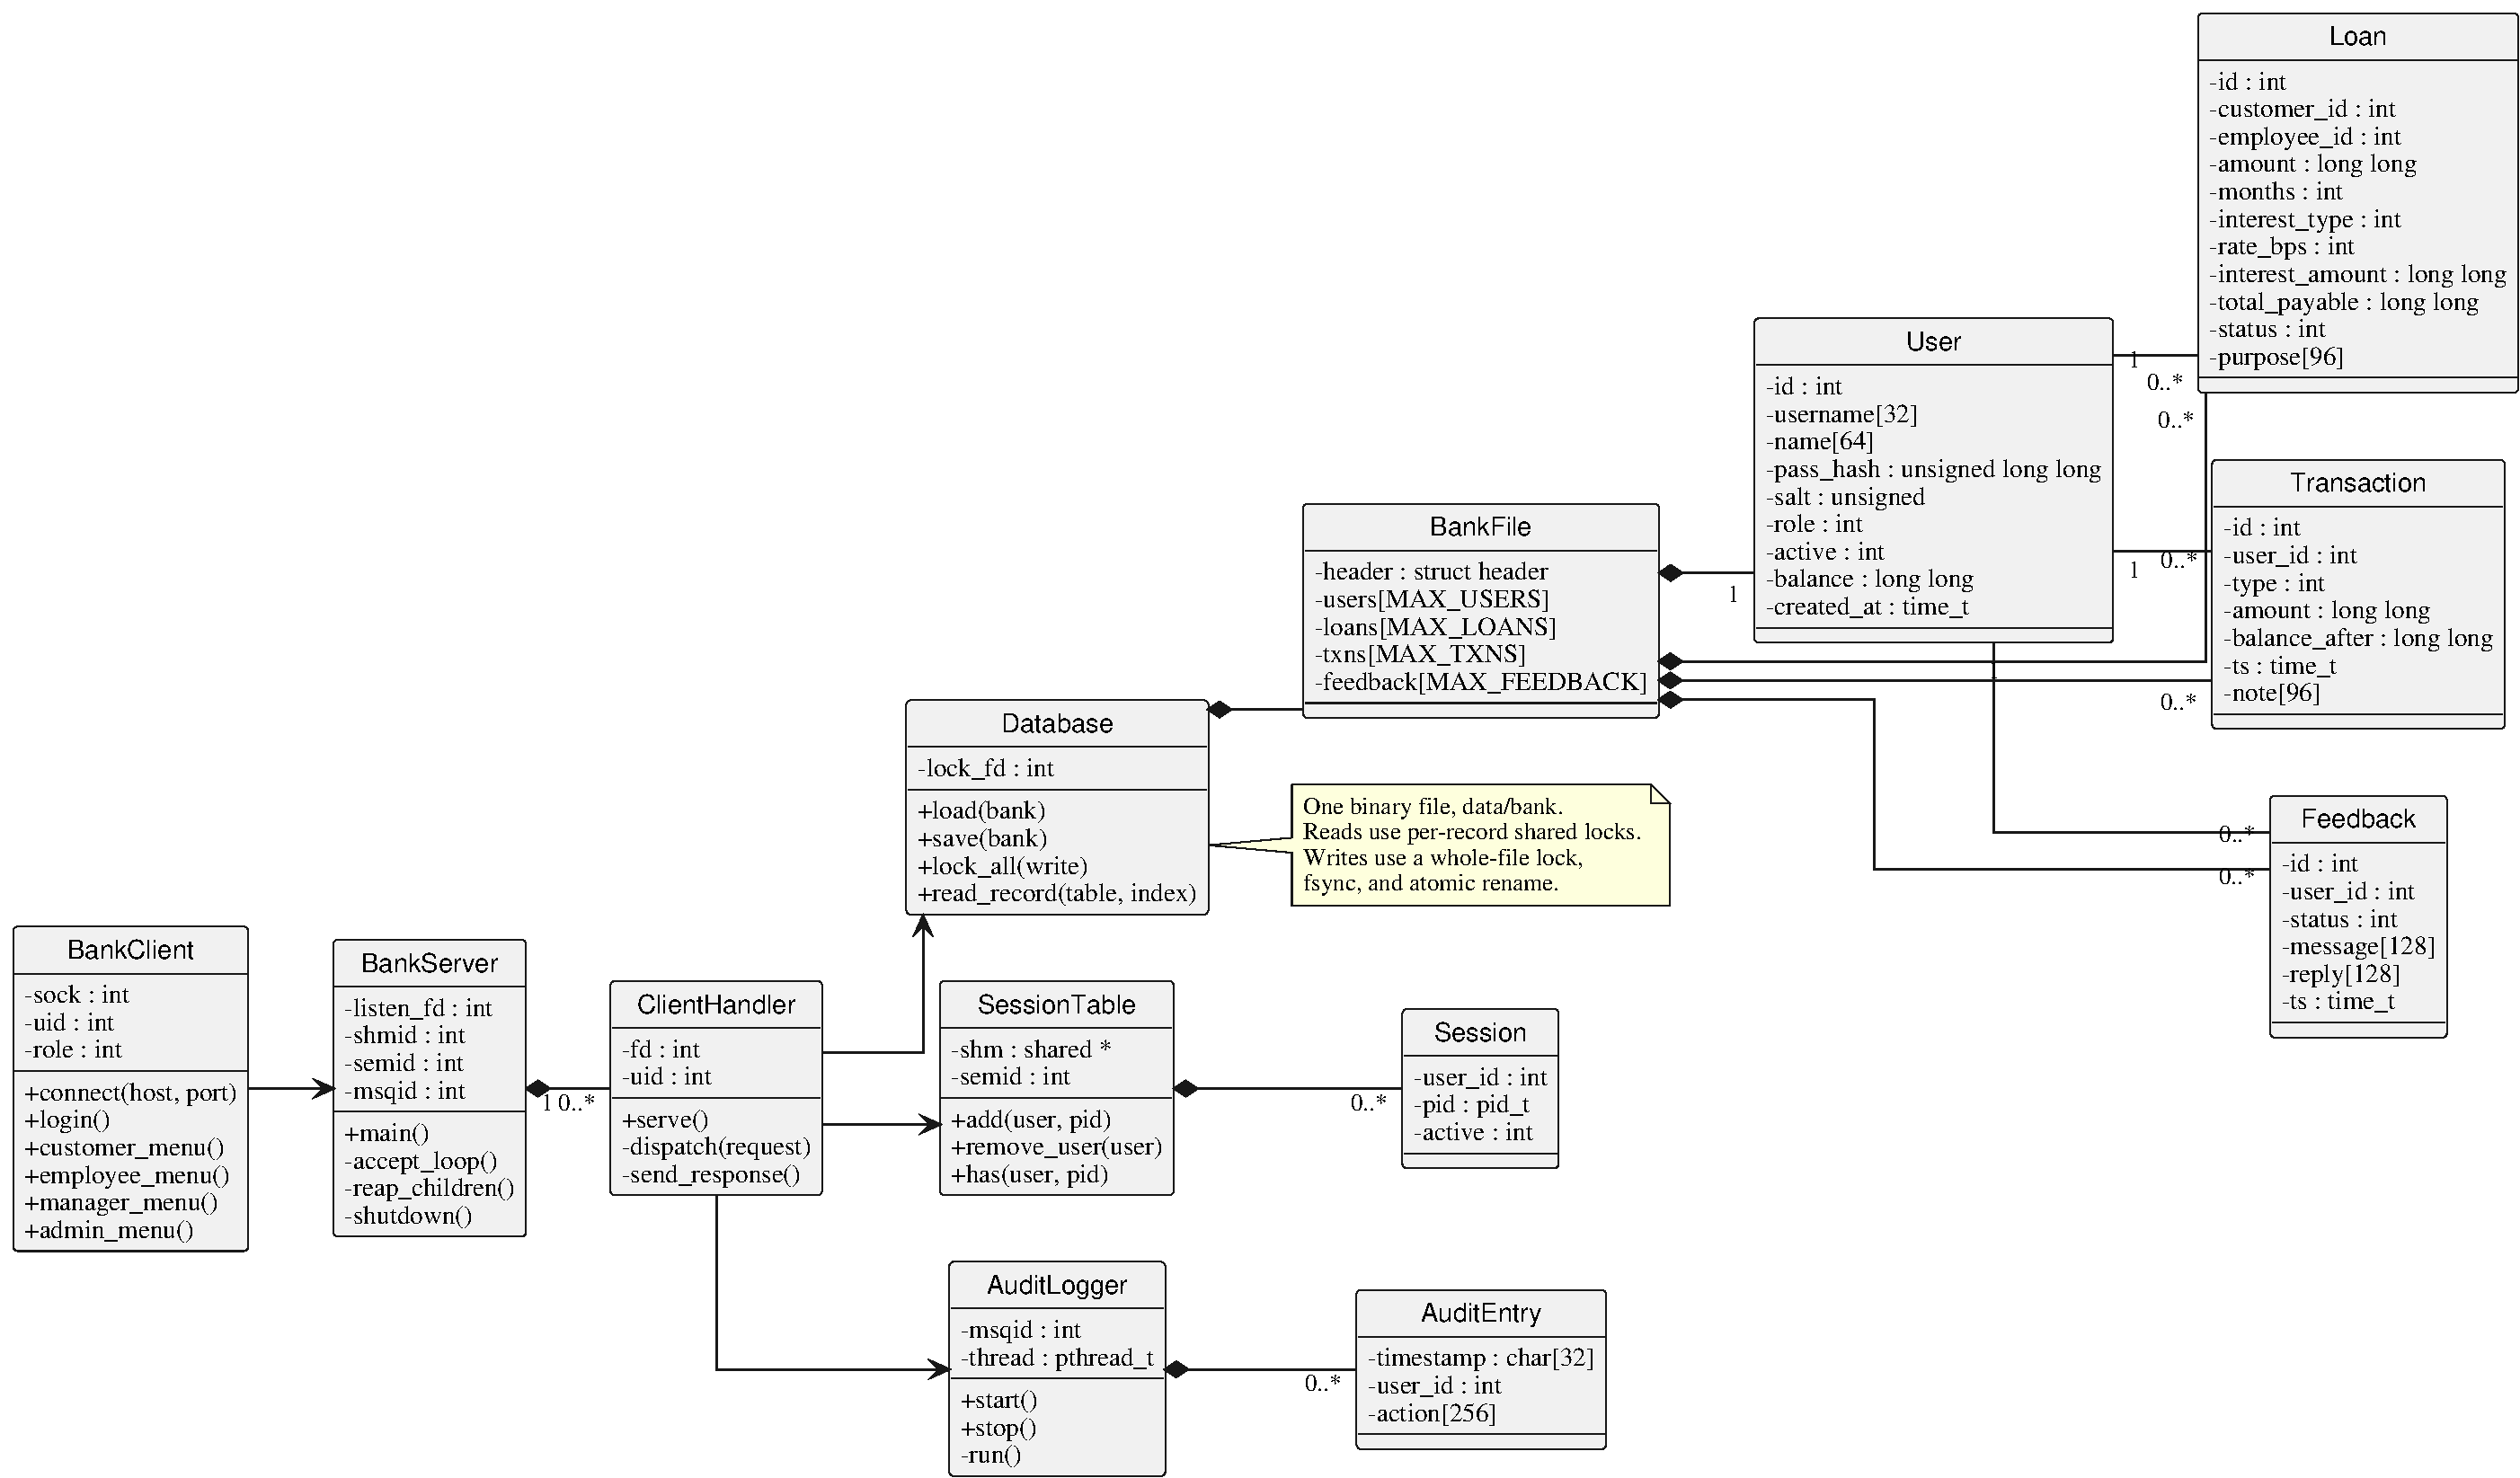
\includegraphics[width=0.98\linewidth]{class_diagram.pdf}
\caption{Complete class structure. Roles are stored in the user record and checked by the handler dispatch.}
  \label{fig:class-full}
\end{figure}

\texttt{BankClient} manages the socket and menus. \texttt{BankServer} manages the listening socket and IPC objects. \texttt{ClientHandler} runs one connection and dispatches requests. \texttt{Database} provides the data file and lock helpers, \texttt{SessionTable} provides the shared memory and semaphore, and \texttt{AuditLogger} provides the message queue and logger thread. The record classes map directly to the arrays in \texttt{struct bank}.

\subsection{Sequence diagrams}

Figure~\ref{fig:seq-login} covers login and one session per user. Figure~\ref{fig:seq-transfer} follows a transfer with the whole-file write lock and atomic rename, and Figure~\ref{fig:seq-loan} shows the three-role loan workflow.

\begin{figure}[H]
  \centering
  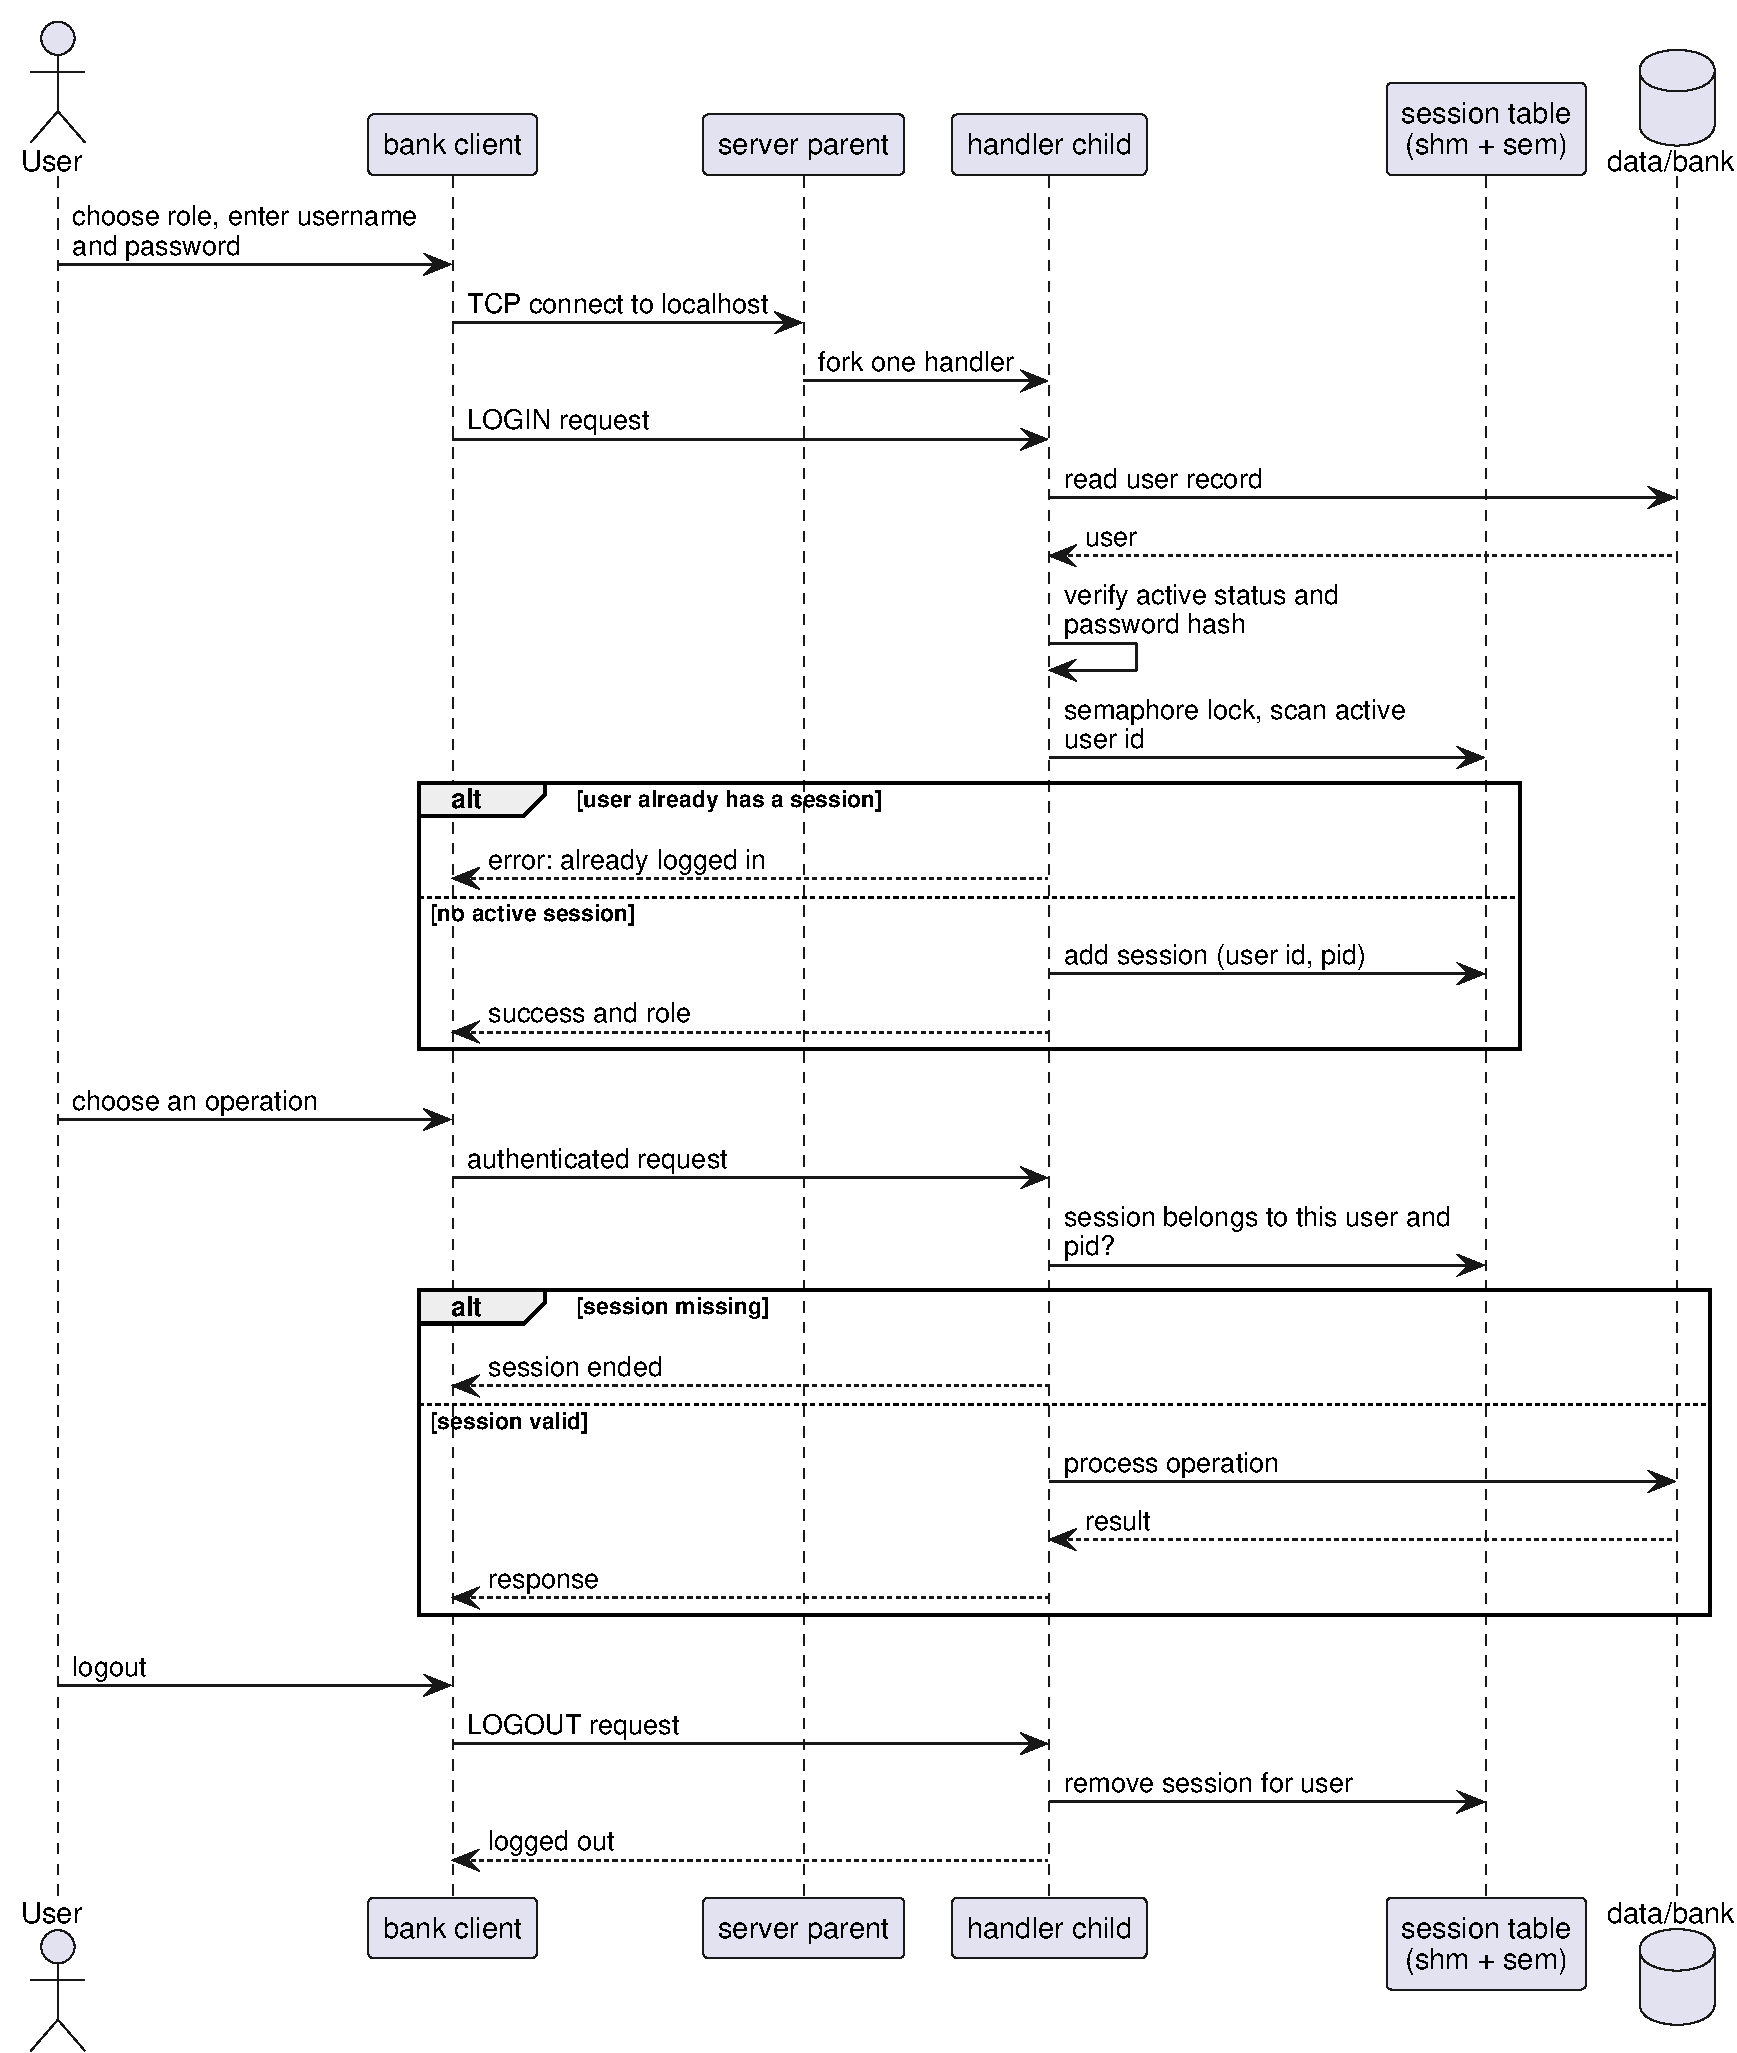
\includegraphics[width=0.82\linewidth]{sequence_login.pdf}
\caption{Login and one session per user.}
  \label{fig:seq-login}
\end{figure}

\begin{figure}[H]
  \centering
  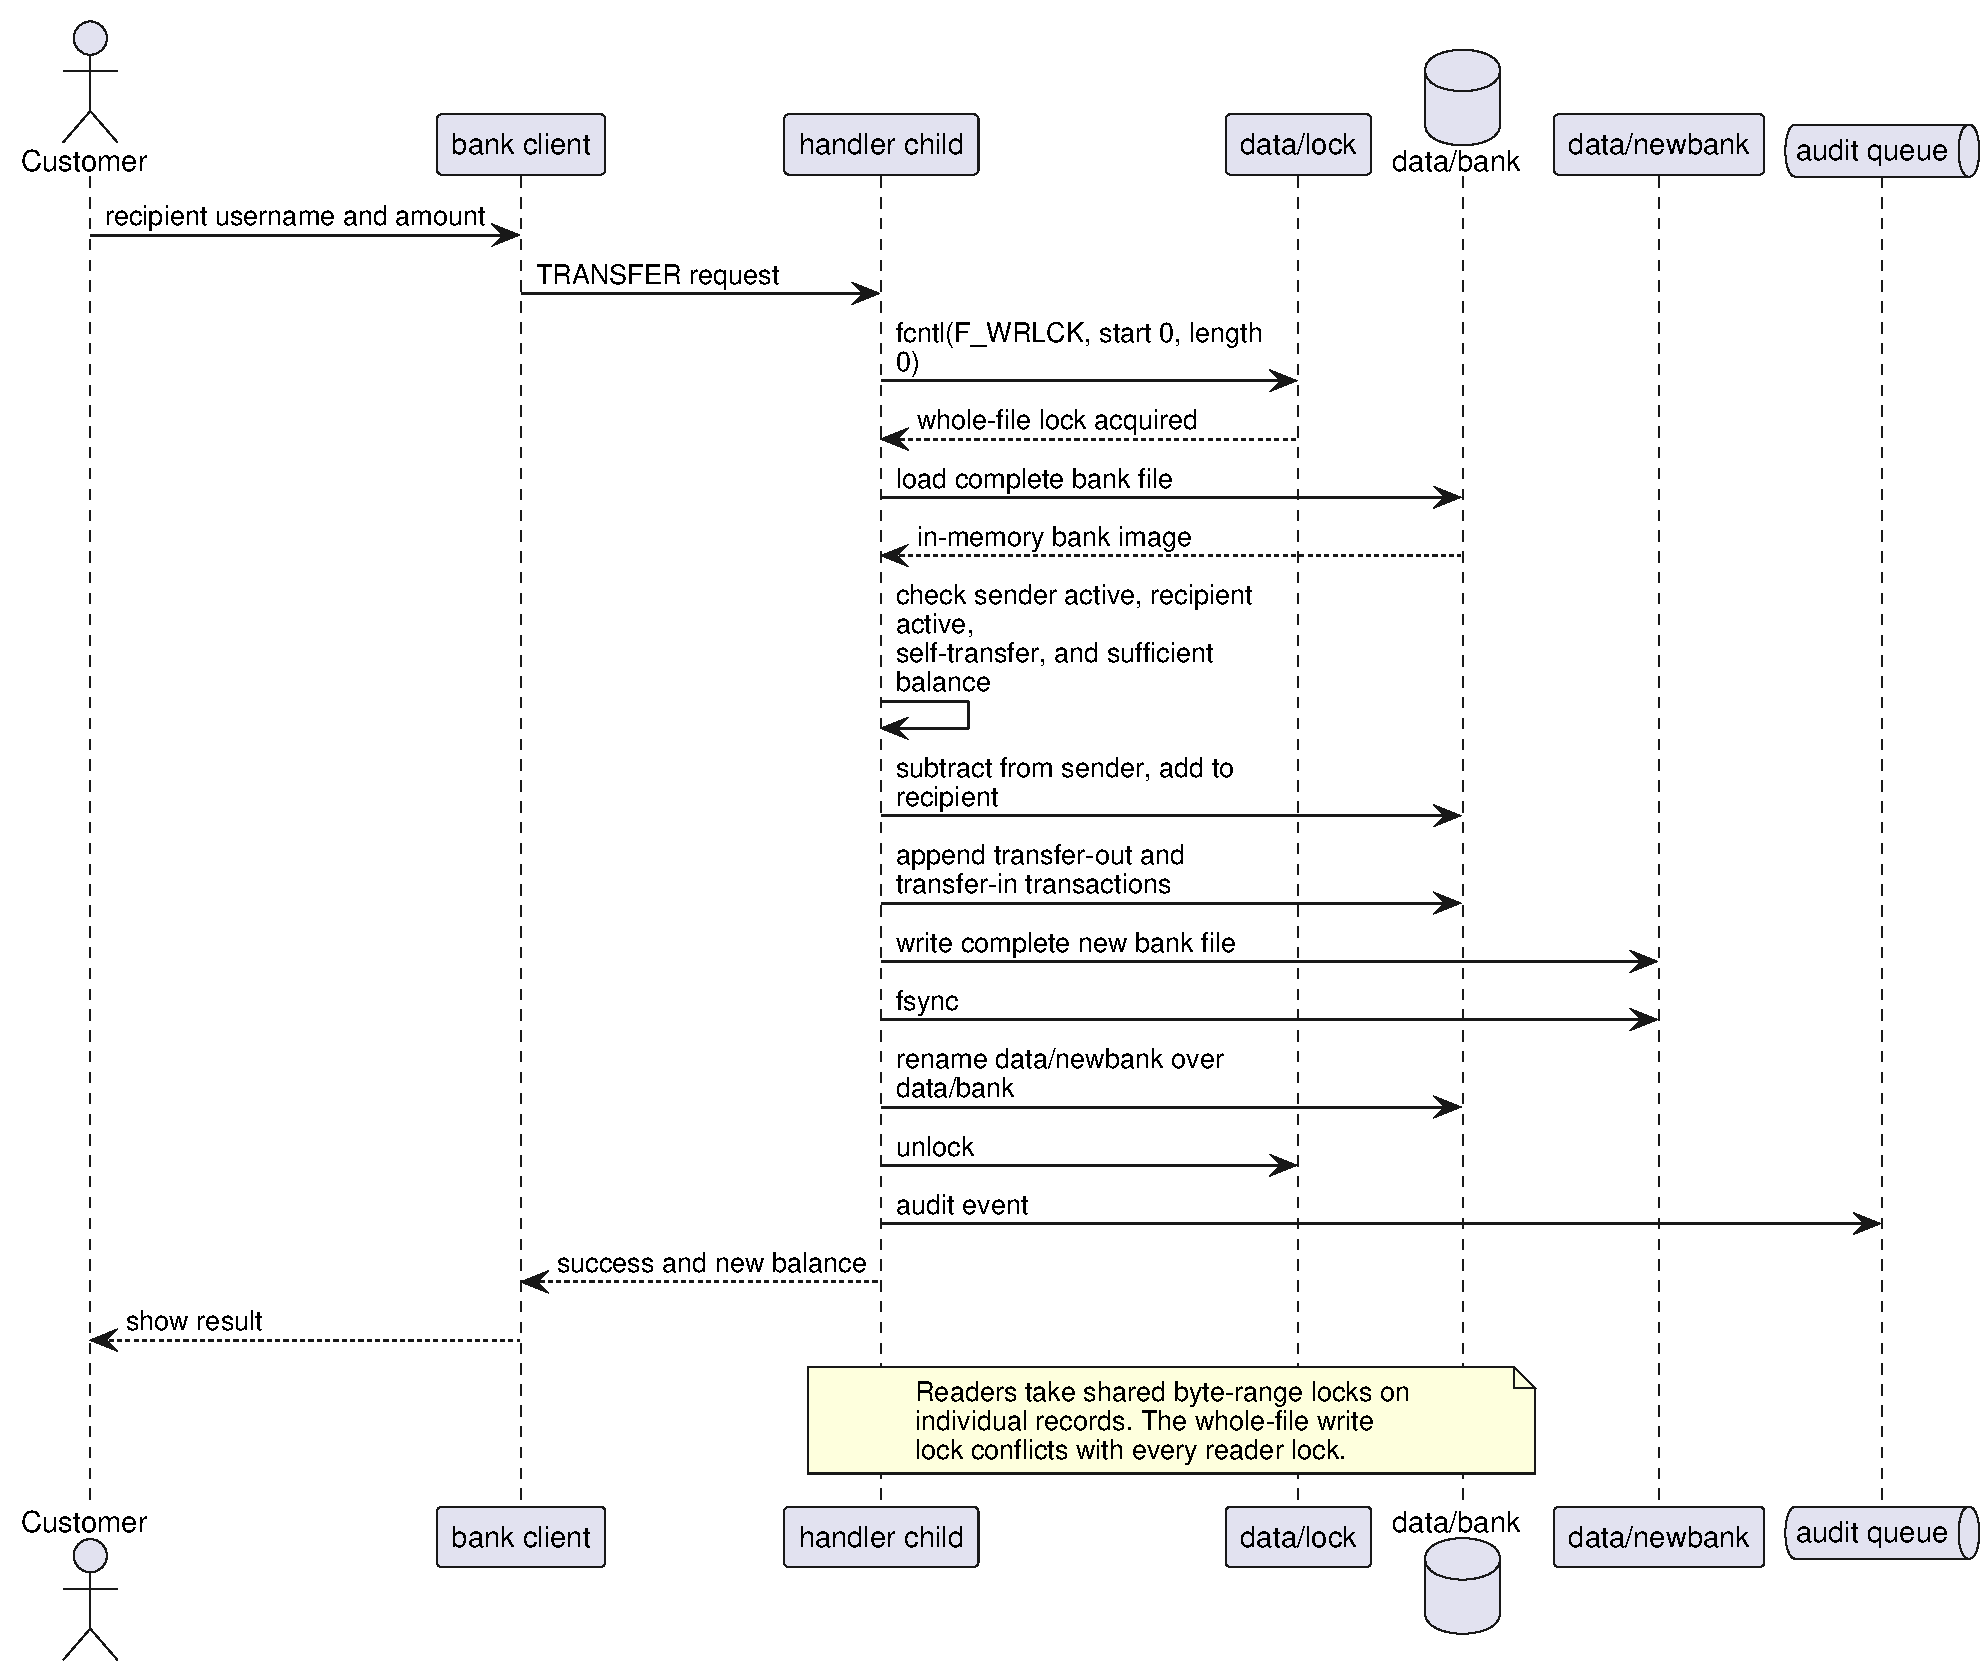
\includegraphics[width=0.92\linewidth]{sequence_transfer.pdf}
\caption{Atomic transfer with a whole-file write lock.}
  \label{fig:seq-transfer}
\end{figure}

\begin{figure}[H]
  \centering
  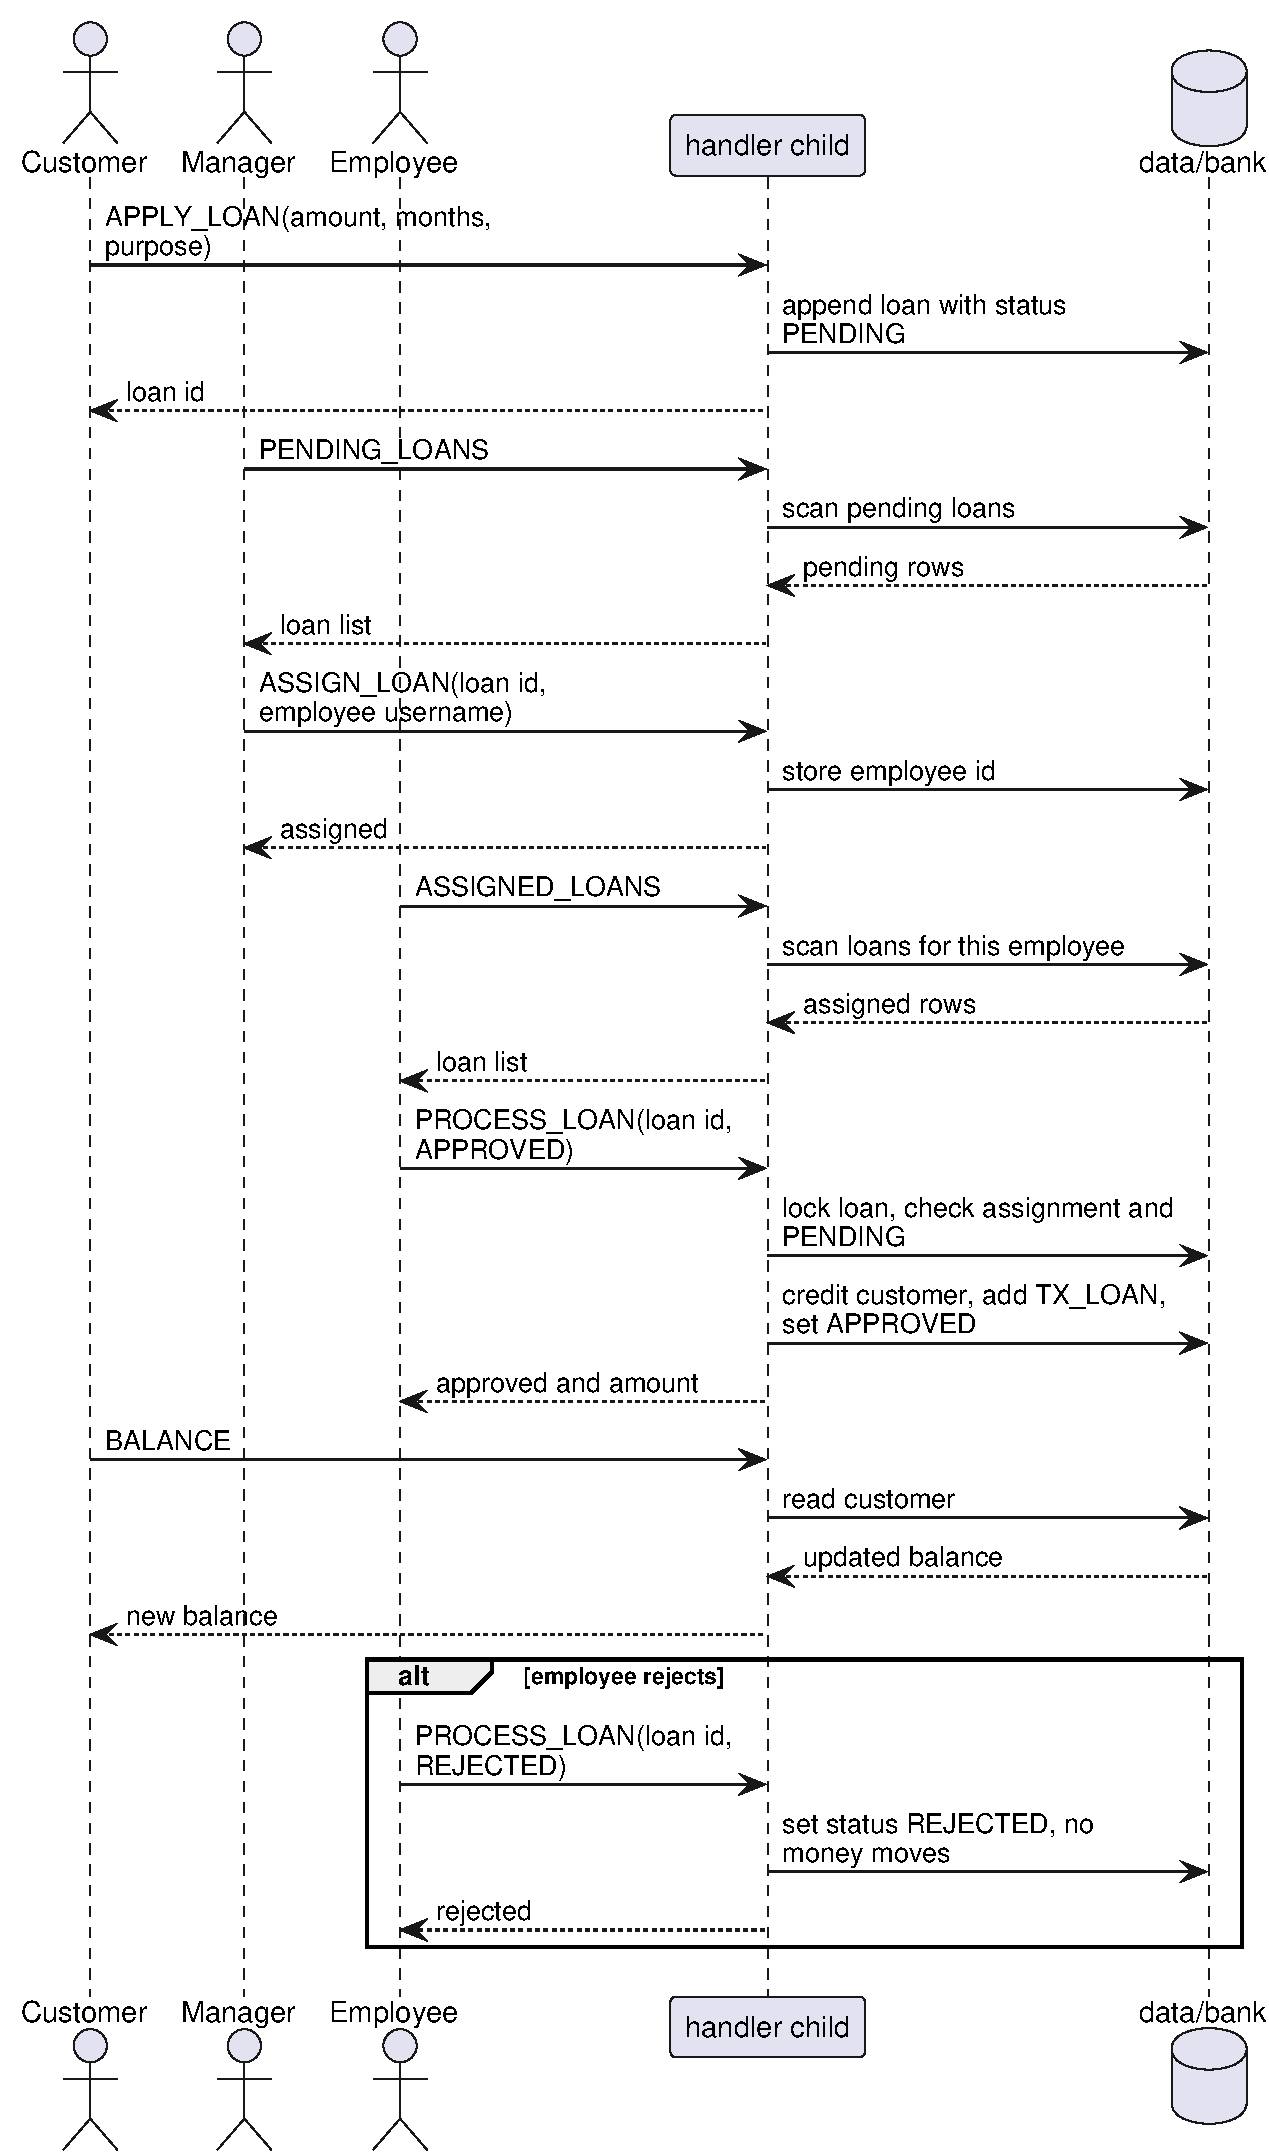
\includegraphics[width=0.62\linewidth]{sequence_loan.pdf}
\caption{Loan application, assignment, and decision.}
  \label{fig:seq-loan}
\end{figure}

\section{Implementation}
\label{sec:implementation}

\subsection{Project Structure}

The implementation is split into three layers. The shared layer includes storage, locking, sockets, sessions, and audit. The server layer includes the role handlers for customer, employee, manager, and administrator activity. The client layer includes the terminal menus.

\begin{longtable}{L{0.24\linewidth}L{0.64\linewidth}}
\hline
Path & Responsibility \\
\hline
\endhead
\texttt{include/} & Records, protocol, database, IPC, socket, server helper, and handler declarations. \\
\texttt{src/common/} & \texttt{db.c} file storage and locking, \texttt{ipc.c} sessions and audit, \texttt{util.c} shared money and write helpers, \texttt{net.c} send and receive loops. \\
\texttt{src/server/} & \texttt{server.c} process and socket loop, \texttt{dispatch.c} request routing, and the domain modules \texttt{auth.c}, \texttt{accounts.c}, \texttt{transactions.c}, \texttt{customers.c}, \texttt{loans.c}, \texttt{feedback.c}, and \texttt{admin.c}. \\
\texttt{src/client/} & \texttt{client.c} role menus, prompts, and local menu state. \\
\texttt{Makefile} & C17 build for both programs. \\
\hline
\end{longtable}

Every request handled by the server follows the following set of steps:
\begin{enumerate}
\item The client formats a \texttt{struct request} and calls \texttt{send\_all} in \texttt{src/common/net.c}.
\item The parent accepts the connection in \texttt{src/server/server.c} and forks one child. The child calls \texttt{handle\_request} in \texttt{src/server/dispatch.c}.
\item The dispatcher checks the session with \texttt{session\_has} in \texttt{src/common/ipc.c}, then checks the active flag and the role.
\item The handler calls \texttt{begin\_write} and \texttt{end\_write} in \texttt{src/common/util.c}. These functions call \texttt{db\_lock\_all}, \texttt{db\_load}, \texttt{db\_save}, and \texttt{db\_unlock\_all} in \texttt{src/common/db.c}.
\item The client receives the response through \texttt{recv\_all}. The handler also posts an audit event through \texttt{audit\_log}.
\end{enumerate}

\subsection{Customer functions}

The customer menu is implemented in \texttt{src/client/client.c}. Menu item 0 clears the screen. The handlers are in \texttt{src/server/auth.c}, \texttt{src/server/accounts.c}, \texttt{src/server/transactions.c}, \texttt{src/server/loans.c}, and \texttt{src/server/feedback.c}.

\begin{longtable}{L{0.20\linewidth}L{0.23\linewidth}L{0.43\linewidth}}
\hline
Menu item & Handler and file & Behaviour and mechanism \\
\hline
\endhead
Login, main 1 & \texttt{do\_login} in \texttt{auth.c}; \texttt{session\_add} in \texttt{ipc.c} & Checks the password hash and active flag, adds one session slot under the semaphore, refuses a duplicate. \\
View balance, 1 & \texttt{do\_balance} in \texttt{accounts.c} & Reads the user record with a shared lock and prints the balance. \\
Deposit, 2 & \texttt{do\_deposit} in \texttt{accounts.c} & Takes the whole-file write lock, increases the balance, appends a \texttt{DEPOSIT} row, saves, and audits. \\
Withdraw, 3 & \texttt{do\_withdraw} in \texttt{accounts.c} & Rejects a non-positive amount or insufficient balance, decreases the balance, appends a \texttt{WITHDRAW} row, saves, and audits. \\
Transfer, 4 & \texttt{do\_transfer} in \texttt{transactions.c} & Checks the recipient, self-transfer, active status, and balance; changes both balances and adds two ledger rows in one atomic save. \\
Apply for loan, 5 & \texttt{do\_apply\_loan} in \texttt{loans.c} & Validates amount and term, reads the bank-wide rate and method, calculates interest, and stores the principal, rate, interest, and total payable in a \texttt{PENDING} loan. \\
Change password, 6 & \texttt{do\_change\_password} in \texttt{auth.c} & Verifies the old hash, creates a new salt and hash, saves, and audits. \\
View history, 7 & \texttt{do\_history} in \texttt{transactions.c} & Reads the customer's transaction records with shared locks and prints one row per movement. \\
Mini statement, 8 & \texttt{do\_mini} in \texttt{transactions.c} & Computes deposit, withdrawal, and transfer totals and prints the last five rows. \\
Add feedback, 9 & \texttt{do\_add\_feedback} in \texttt{feedback.c} & Appends a feedback message. \\
Feedback replies, 10 & \texttt{do\_my\_feedback} in \texttt{feedback.c} & Reads the customer's feedback records and prints manager replies. \\
Logout, 11 & \texttt{do\_logout} in \texttt{auth.c} & Removes the session and returns to the login menu. \\
Exit, 12 & client exit path & Sends a logout request and closes the socket. \\
Clear screen, 0 & \texttt{src/client/client.c} & Clears the terminal and repaints the menu. \\
\hline
\end{longtable}

\paragraph{Account operations.} Deposit and withdrawal are implemented with \texttt{begin\_write}. The steps are:
\begin{enumerate}
\item \texttt{begin\_write} takes the whole-file write lock and loads the database.
\item The handler checks the amount and the current balance in memory.
\item A successful operation updates the user record and appends one transaction.
\item \texttt{end\_write} writes the complete new file to \texttt{data/newbank}, flushes it, renames it over \texttt{data/bank}, flushes the directory, and releases the lock.
\item If a check fails, the handler calls \texttt{end\_write(b, 0)} and writes nothing.
\end{enumerate}
The balance and the ledger row therefore change in the same file image.

\paragraph{Transfer and race conditions.} One whole-file lock is used for a transfer because it changes two user records and two ledger rows. Under that lock, the handler:
\begin{itemize}
\item checks the sender and recipient;
\item subtracts the amount from the sender and adds it to the recipient;
\item appends an outgoing row for the sender and an incoming row for the recipient;
\item saves once.
\end{itemize}
If any check fails, no file is written. Two simultaneous transfers cannot interleave their updates, and parallel transfers from different customers produce exact final balances.

\paragraph{History, mini statement, and read consistency.} The history and mini statement are read-only. They use \texttt{db\_read\_header} and \texttt{db\_read\_txn}, and each record read takes a shared lock on its byte range. A writer holds the whole-file lock, which conflicts with these shared locks. A reader therefore sees the old complete file or the new complete file, and it cannot read a record while the writer replaces the file.

\paragraph{Loan application, password, and feedback.}
\begin{itemize}
\item A loan application appends a pending record and leaves balances unchanged.
\item A password change verifies the old hash before it writes the new salt and hash.
\item Feedback is an append-only record with an optional manager reply.
\end{itemize}
All three use the same lock, validation, atomic save, and audit path.

\subsection{Bank employee functions}

The employee menu is implemented in \texttt{src/client/client.c}. The handlers are in the \texttt{customers}, \texttt{loans}, \texttt{transactions}, and \texttt{accounts} modules.

\begin{longtable}{L{0.20\linewidth}L{0.23\linewidth}L{0.43\linewidth}}
\hline
Menu item & Handler and file & Behaviour and mechanism \\
\hline
\endhead
Login, main 2 & \texttt{do\_login} in \texttt{auth.c} & Same hash, active flag, and one-session check as every role. \\
Add customer, 1 & \texttt{do\_add\_customer} in \texttt{customers.c} & Rejects a duplicate username, hashes the password, sets the opening balance, and adds an opening deposit row. \\
Modify customer, 2 & \texttt{do\_modify\_customer} in \texttt{customers.c} & Changes the display name and/or resets the password; blank fields are kept. \\
Process loan, 3 & \texttt{do\_assigned\_loans} and \texttt{do\_process\_loan} in \texttt{loans.c} & Lists assigned loans with the stored interest and total, checks the assignment and pending state, then approves or rejects. \\
View customer transactions, 4 & \texttt{do\_customer\_tx} in \texttt{transactions.c} & Reads the target customer's ledger with shared locks. \\
View assigned loans, 5 & \texttt{do\_assigned\_loans} in \texttt{loans.c} & Lists loans whose employee id matches the session user. \\
Close account, 6 & \texttt{do\_close\_account} in \texttt{accounts.c} & Requires zero balance and no pending or approved loan; marks the account inactive and removes its session. \\
Change password, 7 & \texttt{do\_change\_password} in \texttt{auth.c} & Verifies the old password and stores a new salt and hash. \\
Logout, 8 & \texttt{do\_logout} in \texttt{auth.c} & Removes the session. \\
Exit, 9 & client exit path & Logs out and closes the client. \\
Clear screen, 0 & \texttt{src/client/client.c} & Clears the terminal and repaints the menu. \\
\hline
\end{longtable}

\paragraph{Customer administration.}
\begin{itemize}
\item Adding a customer checks the username under the write lock, so two employees cannot create the same name.
\item The opening balance and its opening transaction are part of the same save.
\item Modifying a customer changes only the fields that were supplied.
\item A password reset uses the same salted hash as a self-service change.
\item Closing an account re-checks the balance and loan rows under the write lock, so a transfer or loan decision cannot race with the closure.
\end{itemize}

\paragraph{Loan processing.}
\begin{itemize}
\item The employee can list only the loans assigned to them.
\item A decision checks that the loan is assigned to the logged-in employee and is still pending.
\item Approval credits the principal and adds a loan transaction in the same atomic image. Rejection changes only the status.
\item The rate and interest calculated at application are kept in the loan record if the bank-wide policy changes.
\item Either decision is audited. A second employee cannot decide the same loan, and a repeated decision fails because the loan is no longer pending.
\end{itemize}

\subsection{Manager functions}

The manager handlers are implemented in \texttt{accounts.c}, \texttt{loans.c}, and \texttt{feedback.c}.

\begin{longtable}{L{0.20\linewidth}L{0.23\linewidth}L{0.43\linewidth}}
\hline
Menu item & Handler and file & Behaviour and mechanism \\
\hline
\endhead
Login, main 3 & \texttt{do\_login} in \texttt{auth.c} & Standard login and session check. \\
Activate or deactivate, 1 & \texttt{do\_set\_active} in \texttt{accounts.c} & Changes the active flag under the write lock, saves, and removes the target session when deactivating. \\
View pending loans, 2 & \texttt{do\_pending\_loans} in \texttt{loans.c} & Reads pending loan records with shared locks. \\
Assign loan, 3 & \texttt{do\_assign\_loan} in \texttt{loans.c} & Checks pending state and an active employee, then stores the employee id. \\
Review feedback, 4 & \texttt{do\_list\_feedback} and \texttt{do\_review\_feedback} in \texttt{feedback.c} & Lists feedback, marks one reviewed, and stores the reply. \\
Change password, 5 & \texttt{do\_change\_password} in \texttt{auth.c} & Verifies the old password and stores a new one. \\
Logout, 6 and exit, 7 & \texttt{do\_logout} in \texttt{auth.c} & Removes the session; exit also closes the client. \\
Clear screen, 0 & \texttt{src/client/client.c} & Clears the terminal and repaints the menu. \\
\hline
\end{longtable}

\paragraph{Account control and session revocation.}
\begin{itemize}
\item Deactivation calls \texttt{session\_remove\_user} after it saves the user record under the write lock.
\item The old client may still hold its socket, but its next request fails the session check.
\item Reactivation changes the same flag back, so the customer can log in again.
\end{itemize}

\paragraph{Loan assignment and feedback.}
\begin{itemize}
\item For loan assignment, it is first checked that the loan is pending and the employee is active; then the employee id is written into the record.
\item The employee's assigned-loan list then shows the loan.
\item Feedback review marks the record and stores a reply. The customer reads it through the feedback view.
\item Both paths use the shared atomic save and audit.
\end{itemize}

\subsection{Administrator functions}

The administrator handlers are implemented in \texttt{admin.c}, with login and password in \texttt{auth.c}.

\begin{longtable}{L{0.20\linewidth}L{0.23\linewidth}L{0.43\linewidth}}
\hline
Menu item & Handler and file & Behaviour and mechanism \\
\hline
\endhead
Login, main 4 & \texttt{do\_login} in \texttt{auth.c} & Standard login and session check. \\
Add employee or manager, 1 & \texttt{do\_add\_employee} in \texttt{admin.c} & Checks uniqueness, hashes the password, sets the role, and saves. \\
Modify user, 2 & \texttt{do\_modify\_user} in \texttt{admin.c} & Changes a name and/or resets a password for any user. \\
Manage roles, 3 & \texttt{do\_set\_role} in \texttt{admin.c} & Changes a user among customer, employee, manager, and administrator; rejects a self-change and removes the target session. \\
List users, 4 & \texttt{do\_list\_users} in \texttt{admin.c} & Reads user records and prints id, username, name, role, status, and balance. \\
View activity log, 5 & \texttt{do\_view\_log} in \texttt{admin.c} & Reads the tail of \texttt{data/audit}. \\
Set loan interest, 6 & \texttt{do\_set\_loan\_rate} in \texttt{admin.c} & Stores one bank-wide annual rate and method in the database header. New loans copy the policy; existing loans keep their stored policy. \\
Change password, 7 & \texttt{do\_change\_password} in \texttt{auth.c} & Verifies the old password and stores a new one. \\
Logout, 8 and exit, 9 & \texttt{do\_logout} in \texttt{auth.c} & Removes the session; exit also closes the client. \\
Clear screen, 0 & \texttt{src/client/client.c} & Clears the terminal and repaints the menu. \\
\hline
\end{longtable}

\paragraph{Loan interest policy.}
\begin{itemize}
\item The administrator sets one annual rate and one method, simple or compound.
\item The initial rate is 0.00\% and the initial method is simple.
\item \texttt{do\_set\_loan\_rate} stores the policy in the database header under the same write lock as other changes.
\item When a customer applies, \texttt{do\_apply\_loan} copies the rate and method into the loan record and calculates the interest and total payable.
\item A later policy change affects only new loans. This snapshot rule keeps the quoted loan terms stable.
\end{itemize}

\paragraph{Role changes and security.}
\begin{itemize}
\item The administrator can change roles but cannot change their own role.
\item A role change saves first and then removes the target session, so the old menu cannot continue with the previous permissions.
\item The user must log in again, and the dispatcher checks the new role.
\end{itemize}

\subsection{Screenshots}

\setlength{\intextsep}{6pt}
\setlength{\abovecaptionskip}{3pt}
\setlength{\belowcaptionskip}{0pt}

\begin{figure}[H]
  \centering
  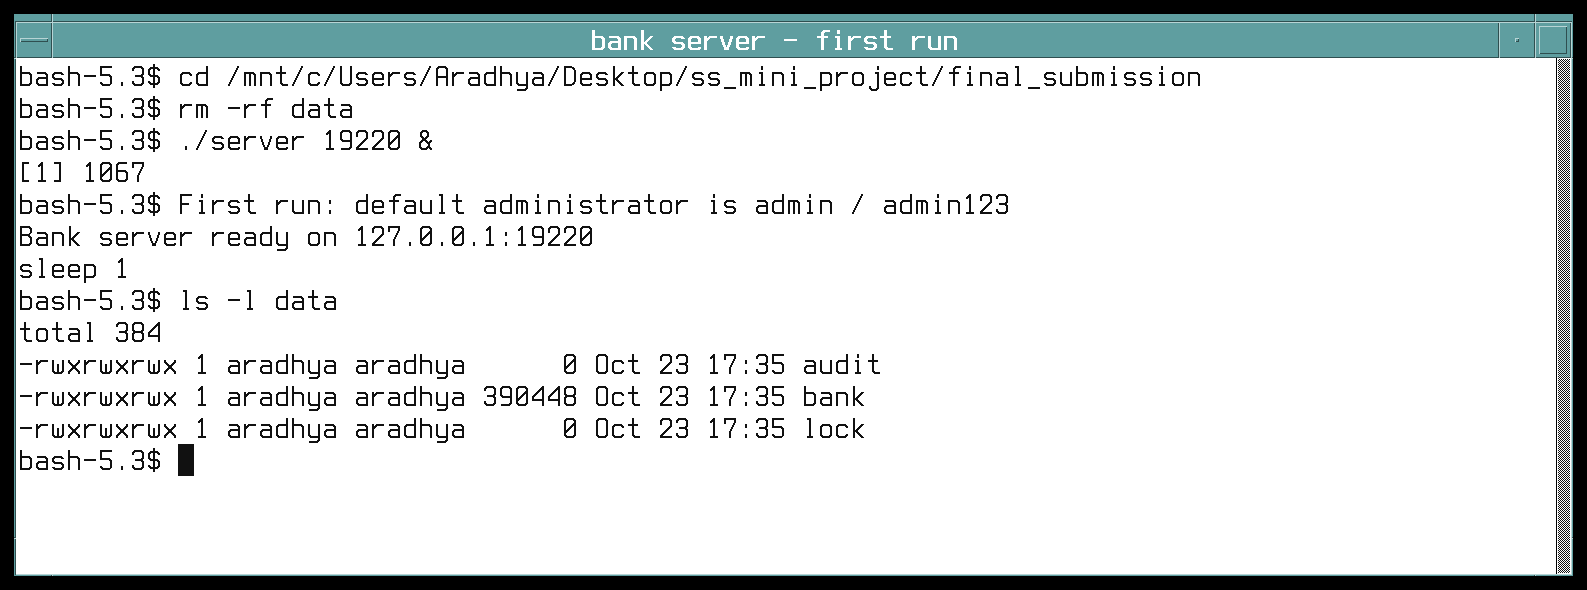
\includegraphics[width=0.64\linewidth]{01_startup.png}
\caption{The first server start and the extensionless data files.}
  \label{fig:startup}
\end{figure}
\begin{figure}[H]
  \centering
  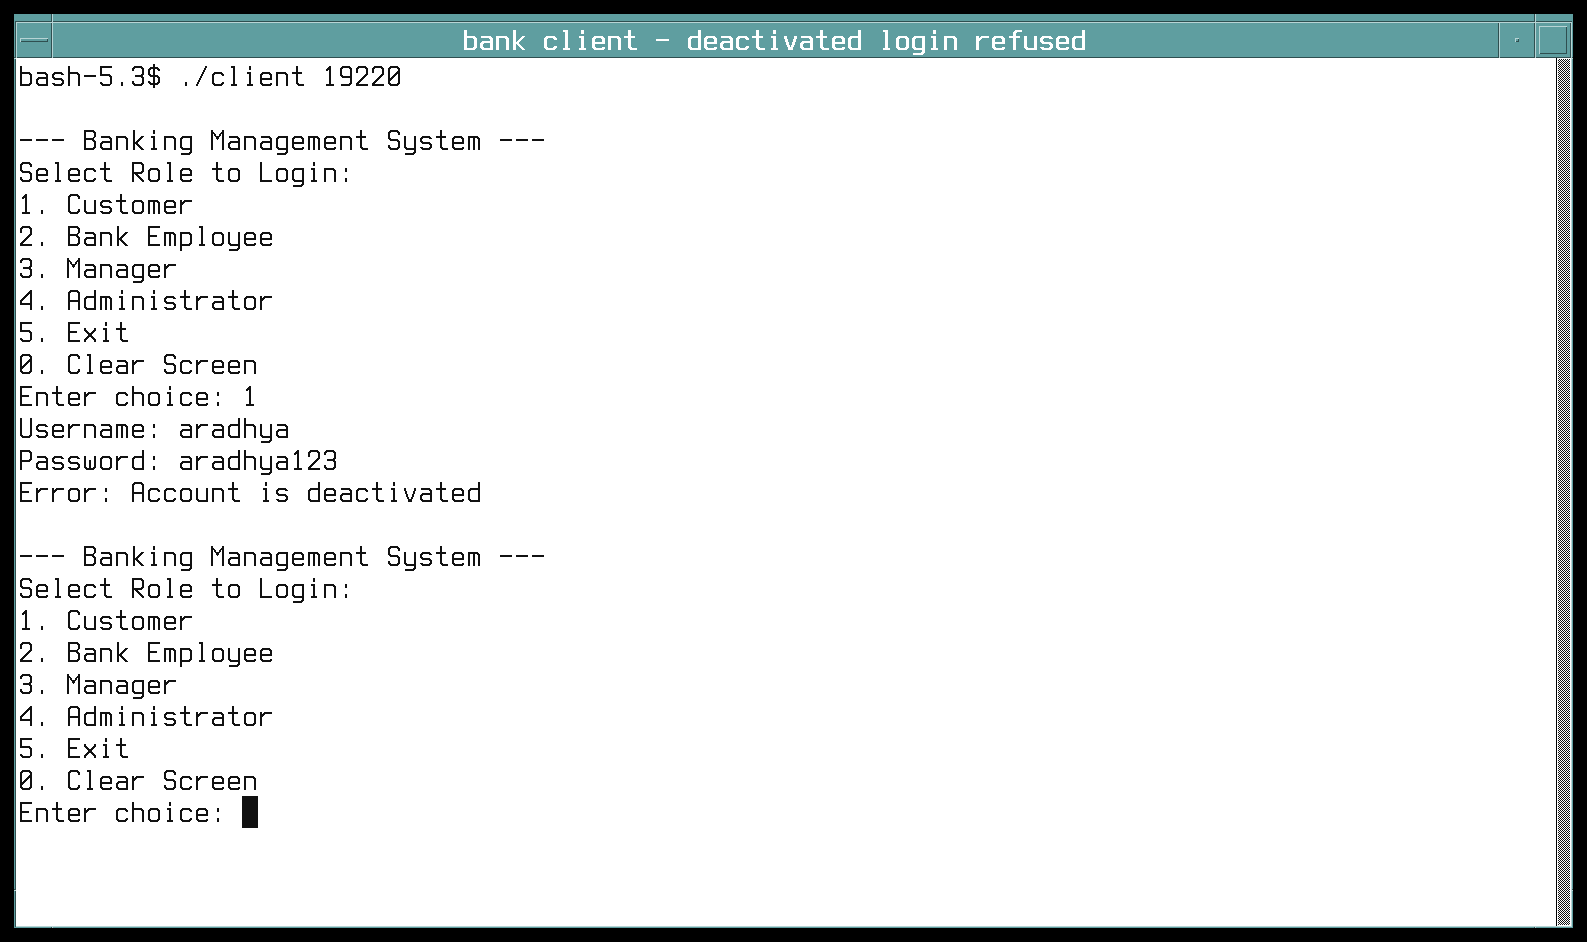
\includegraphics[width=0.64\linewidth]{15_deactivated_login.png}
\caption{The server refuses a deactivated account.}
  \label{fig:deactivated}
\end{figure}
\begin{figure}[H]
  \centering
  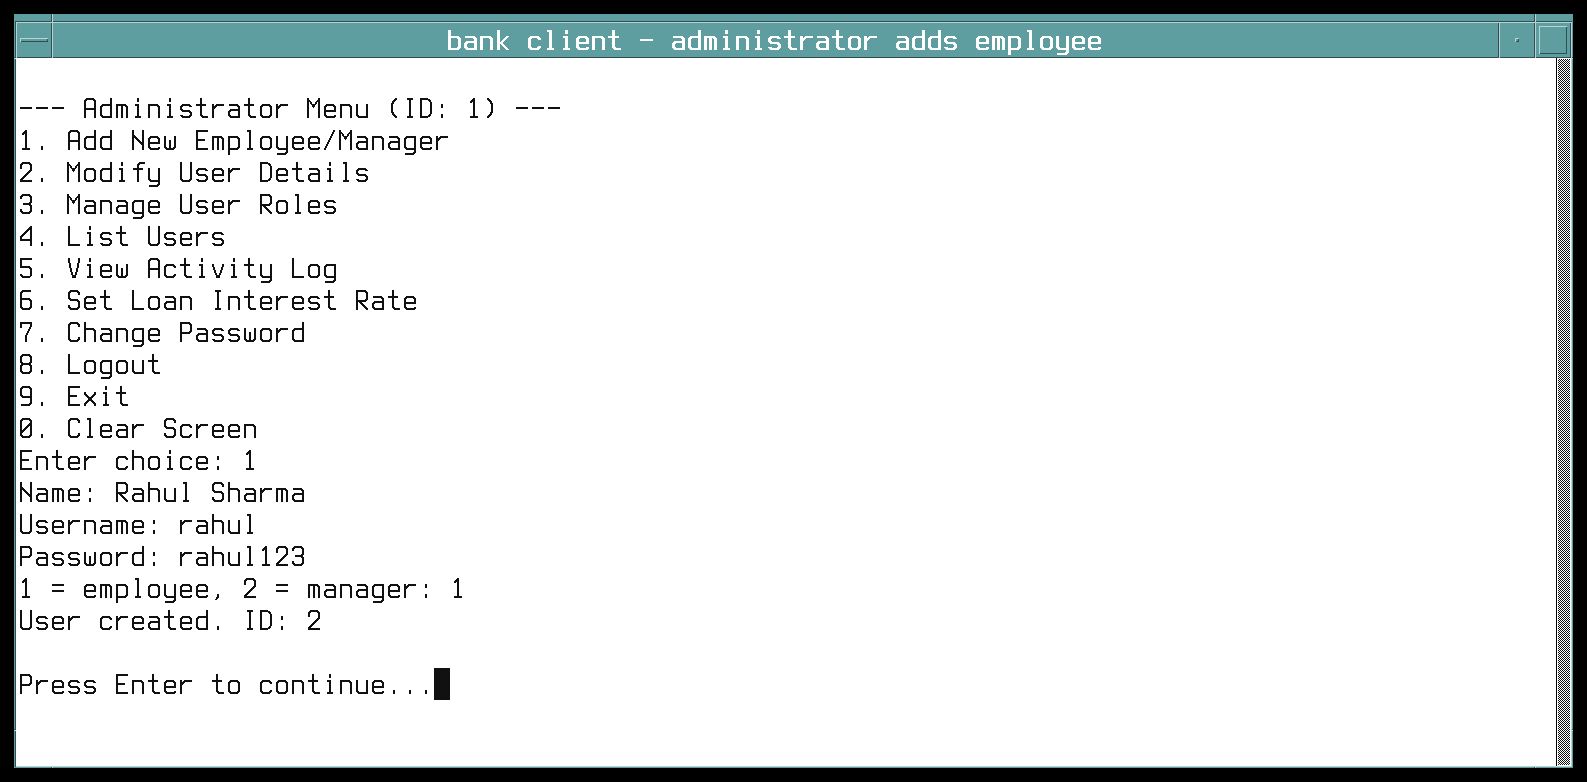
\includegraphics[width=0.64\linewidth]{02_admin_employee.png}
\caption{The administrator adds employee Rahul Sharma.}
  \label{fig:admin-employee}
\end{figure}
\begin{figure}[H]
  \centering
  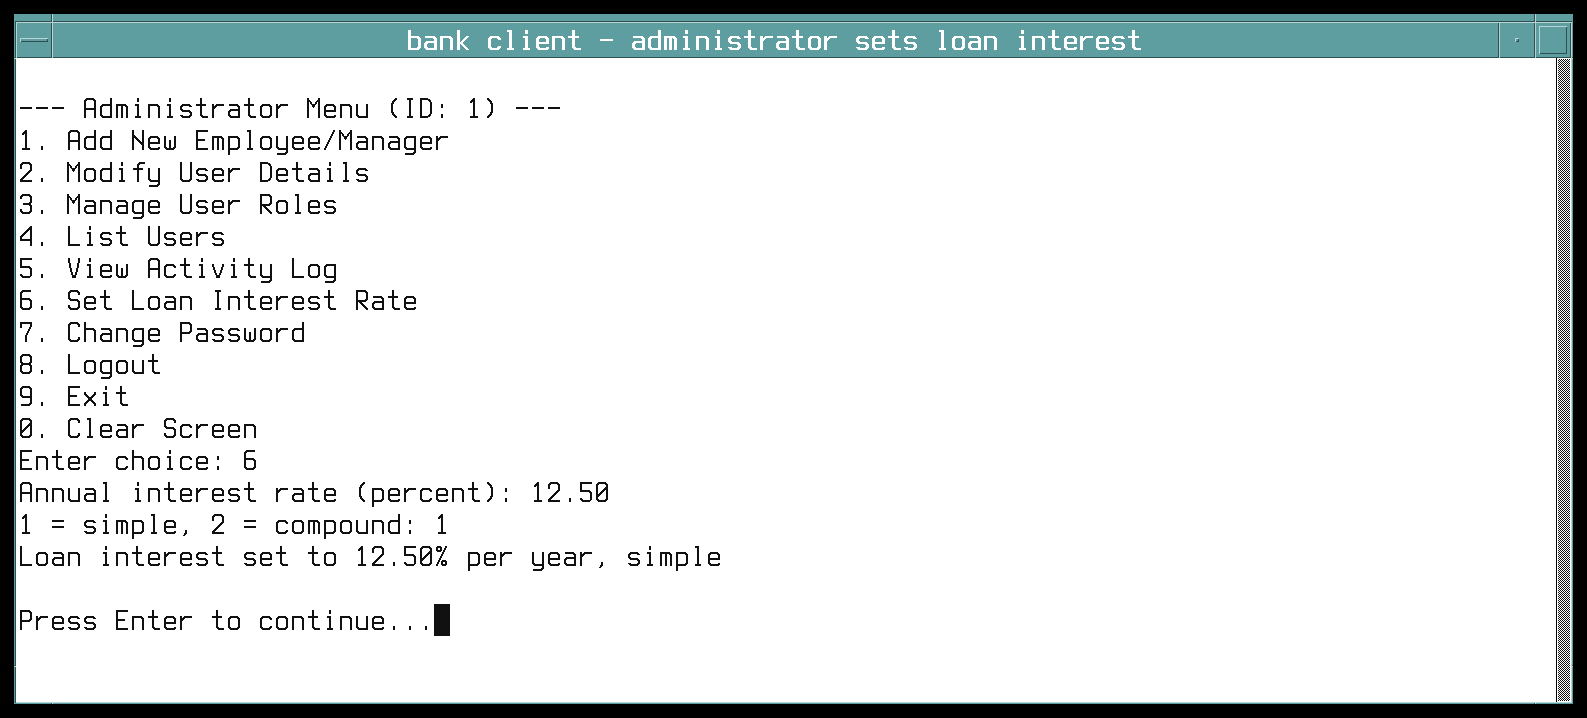
\includegraphics[width=0.64\linewidth]{17_admin_rate.png}
\caption{The administrator sets the bank-wide loan interest policy.}
  \label{fig:admin-rate}
\end{figure}
\begin{figure}[H]
  \centering
  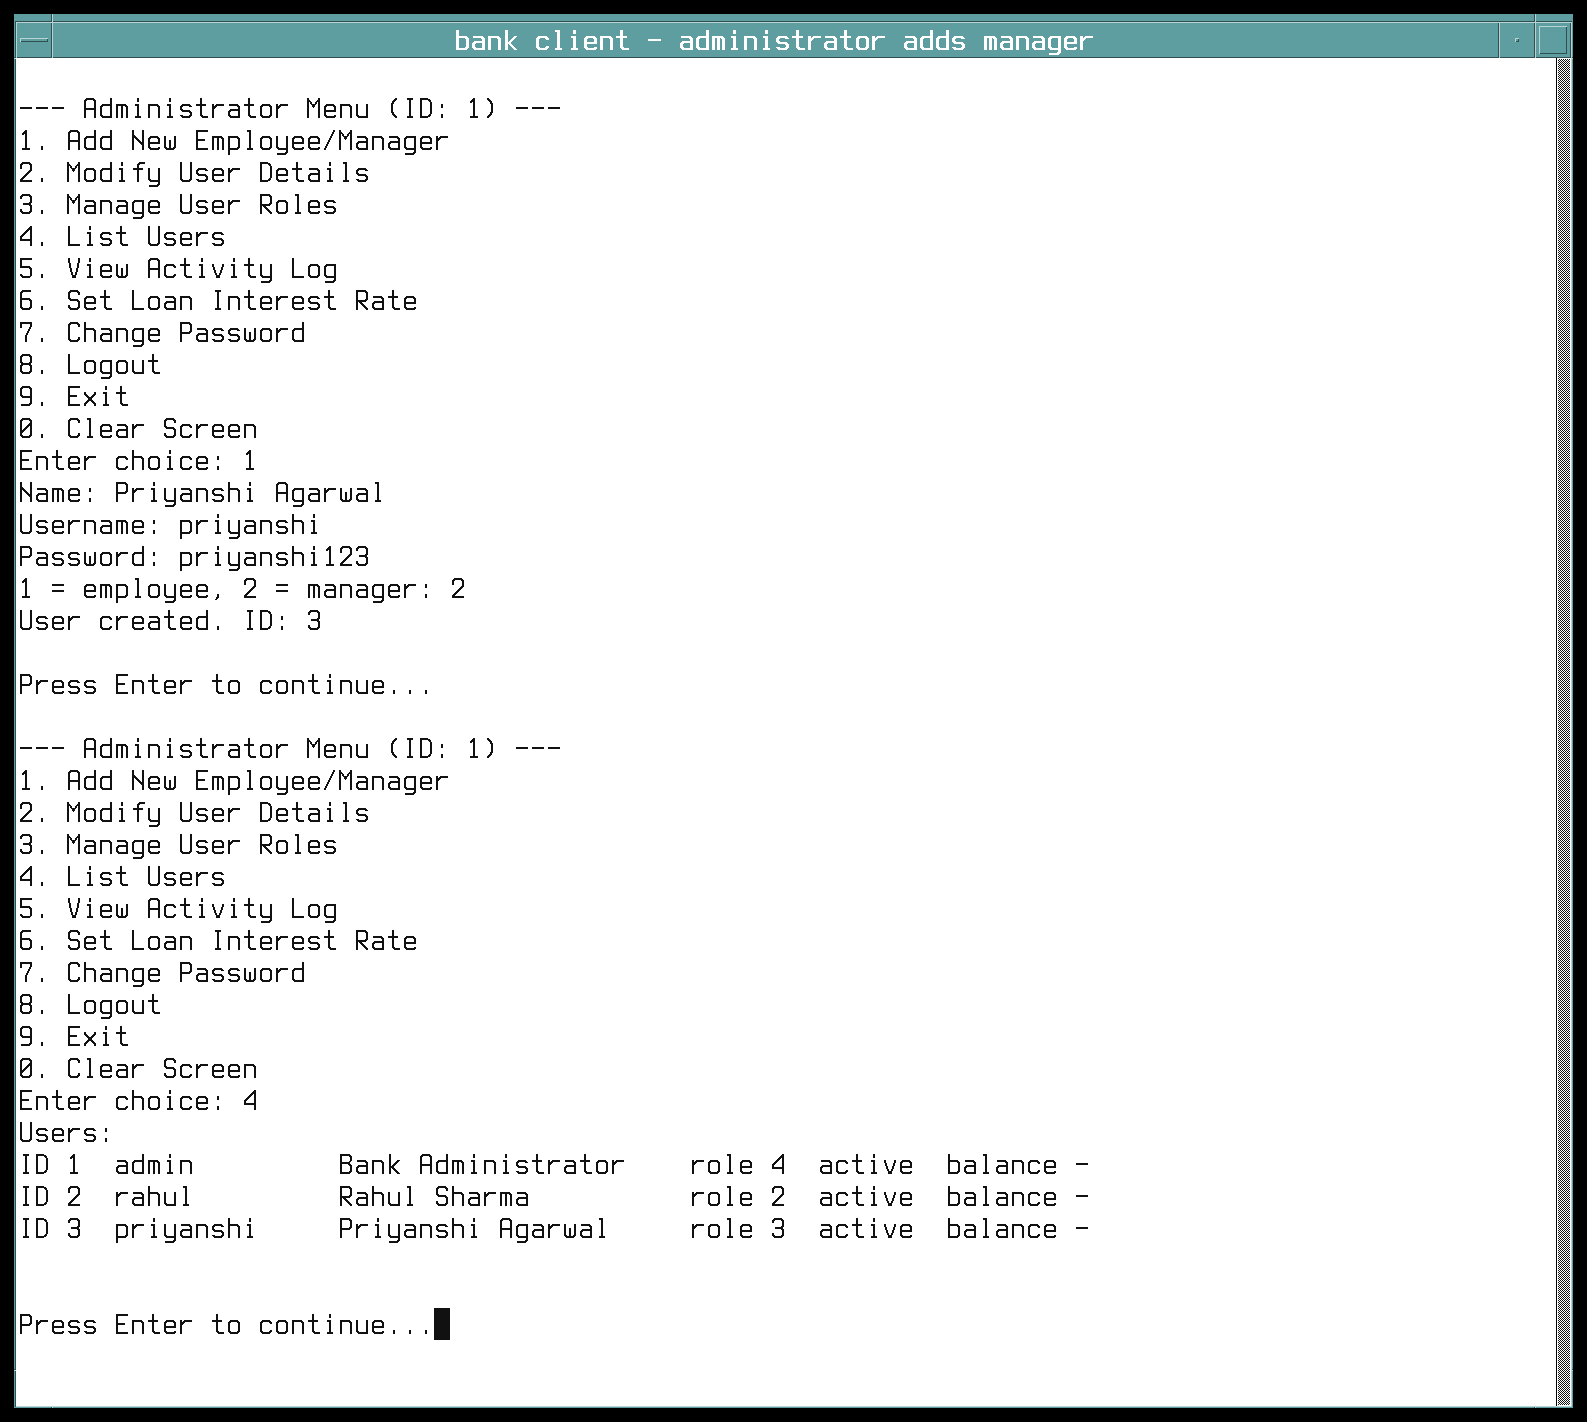
\includegraphics[width=0.64\linewidth]{03_admin_manager.png}
\caption{The administrator adds manager Priyanshi Agarwal.}
  \label{fig:admin-manager}
\end{figure}
\begin{figure}[H]
  \centering
  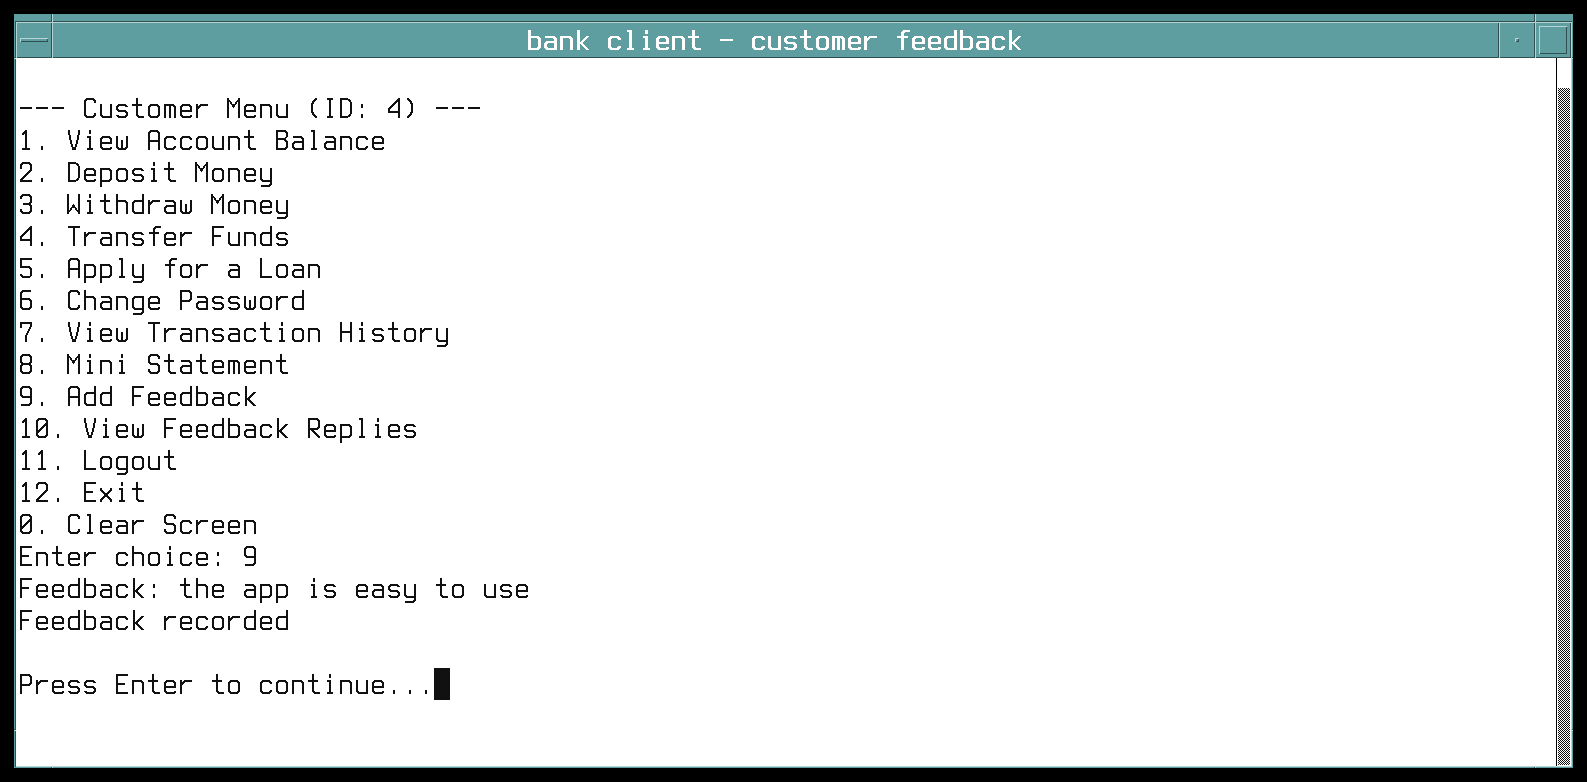
\includegraphics[width=0.64\linewidth]{11_customer_feedback.png}
\caption{The customer submits feedback.}
  \label{fig:customer-feedback}
\end{figure}
\begin{figure}[H]
  \centering
  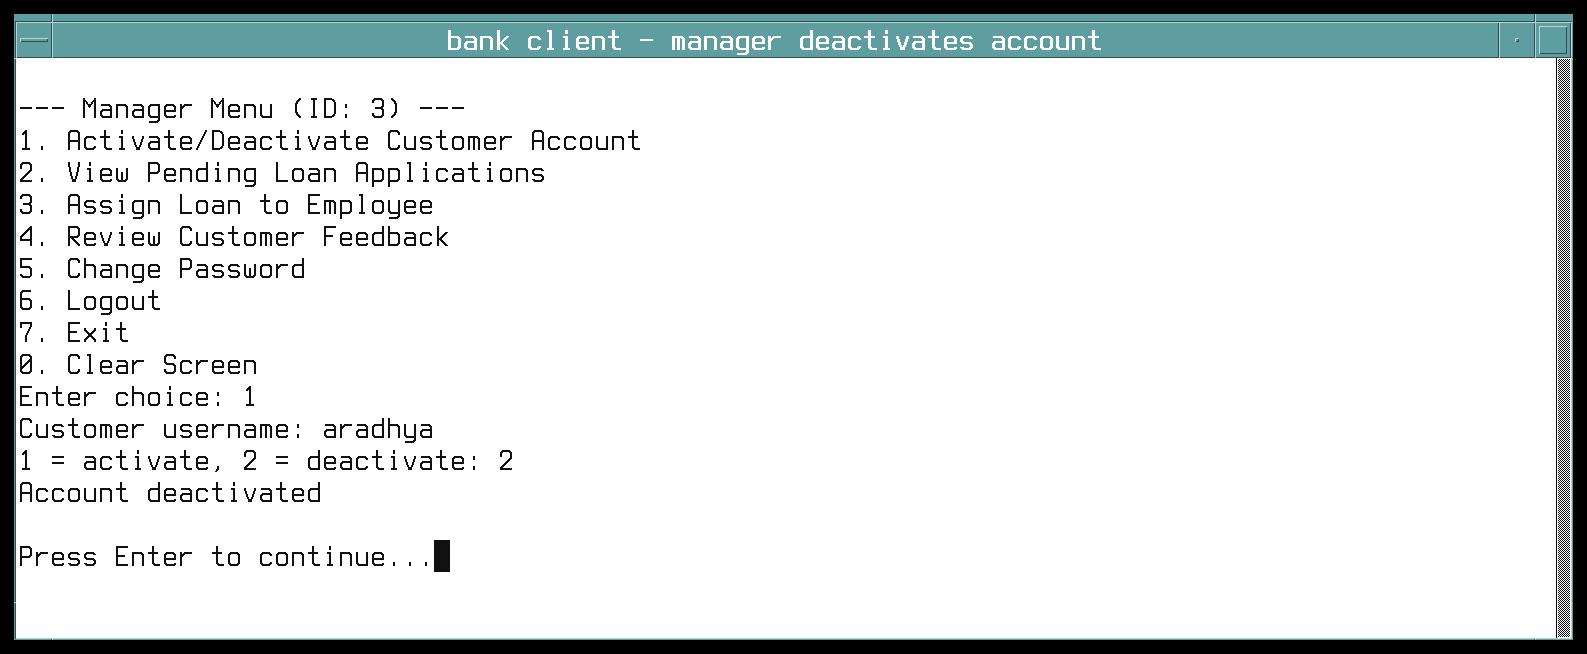
\includegraphics[width=0.64\linewidth]{14_manager_deactivate.png}
\caption{The manager deactivates a customer.}
  \label{fig:manager-deactivate}
\end{figure}
\begin{figure}[H]
  \centering
  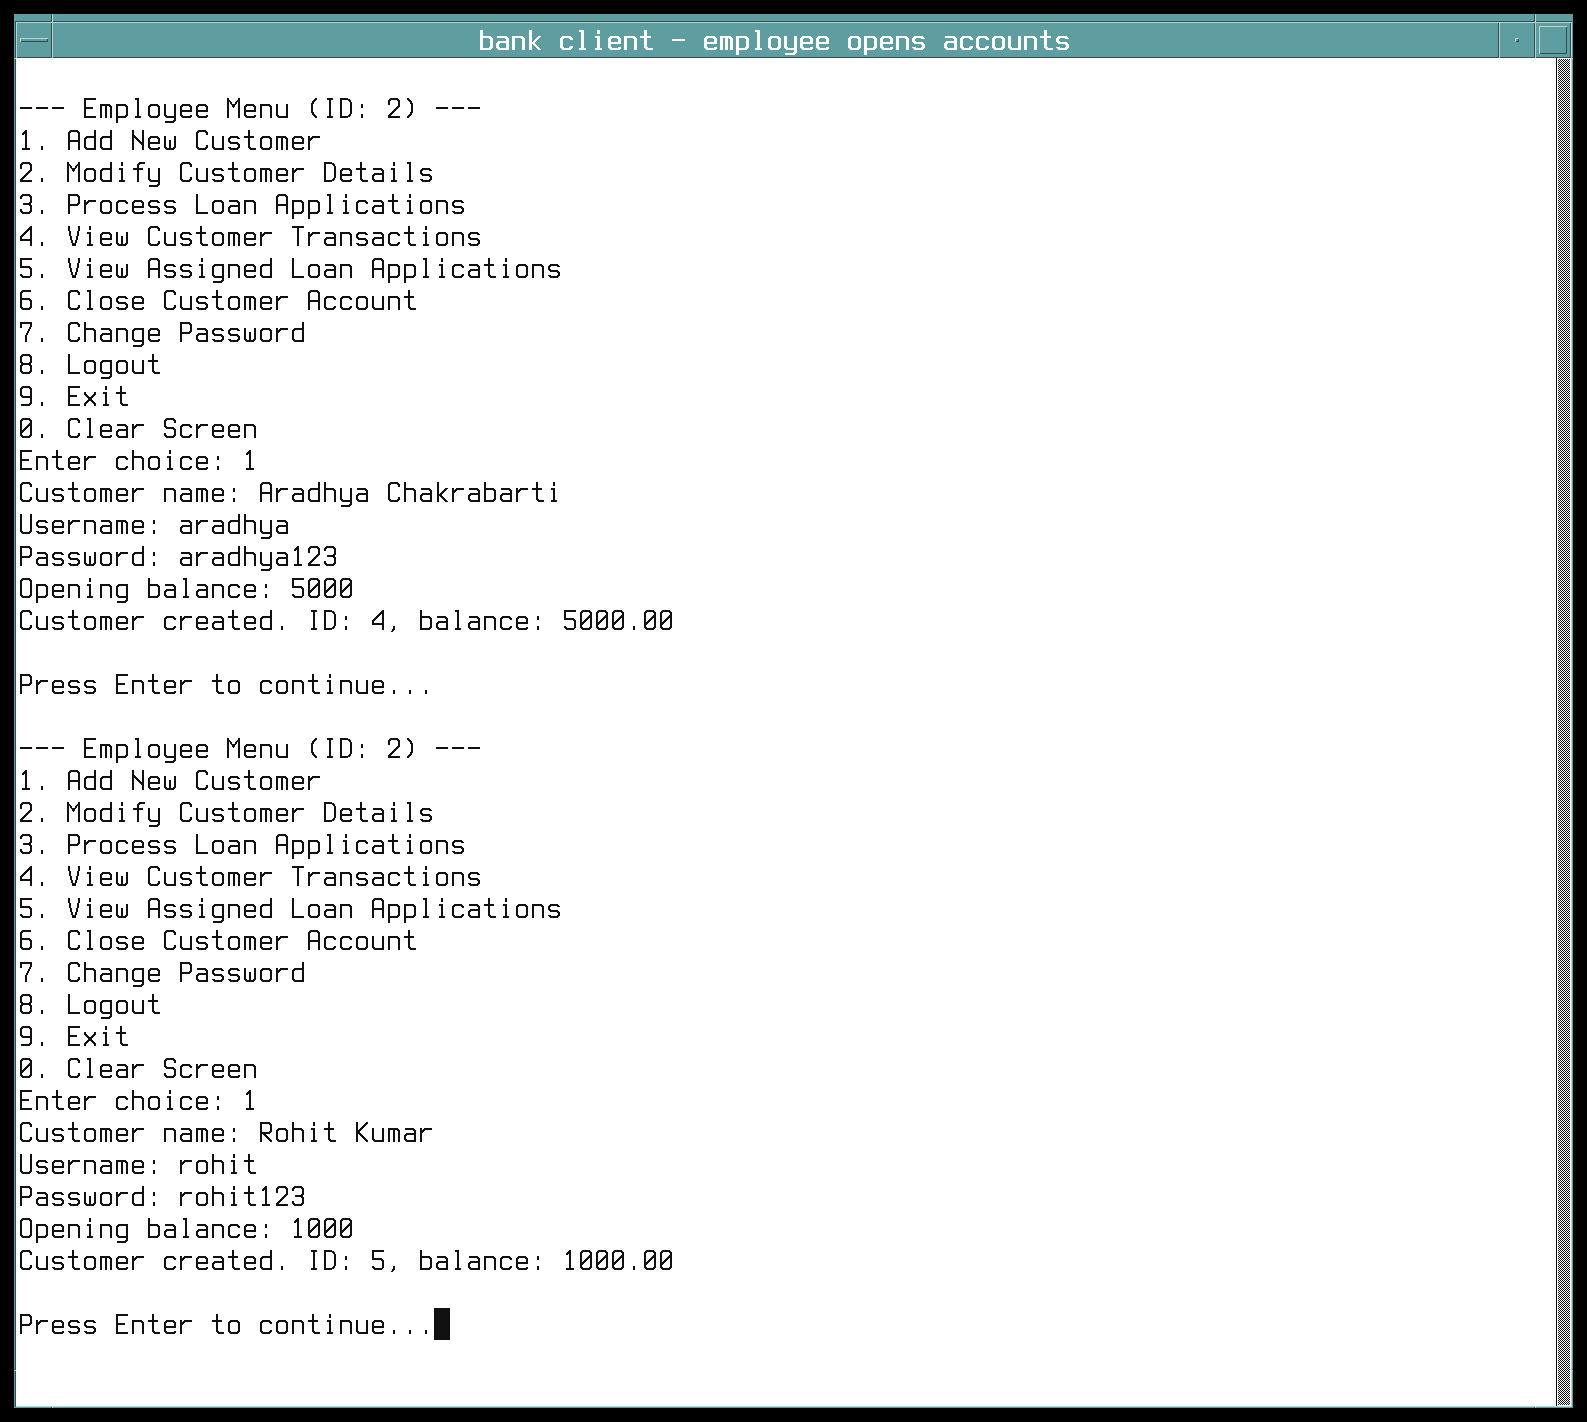
\includegraphics[width=0.64\linewidth]{04_employee_customers.png}
\caption{The employee opens customer accounts.}
  \label{fig:employee-customers}
\end{figure}
\begin{figure}[H]
  \centering
  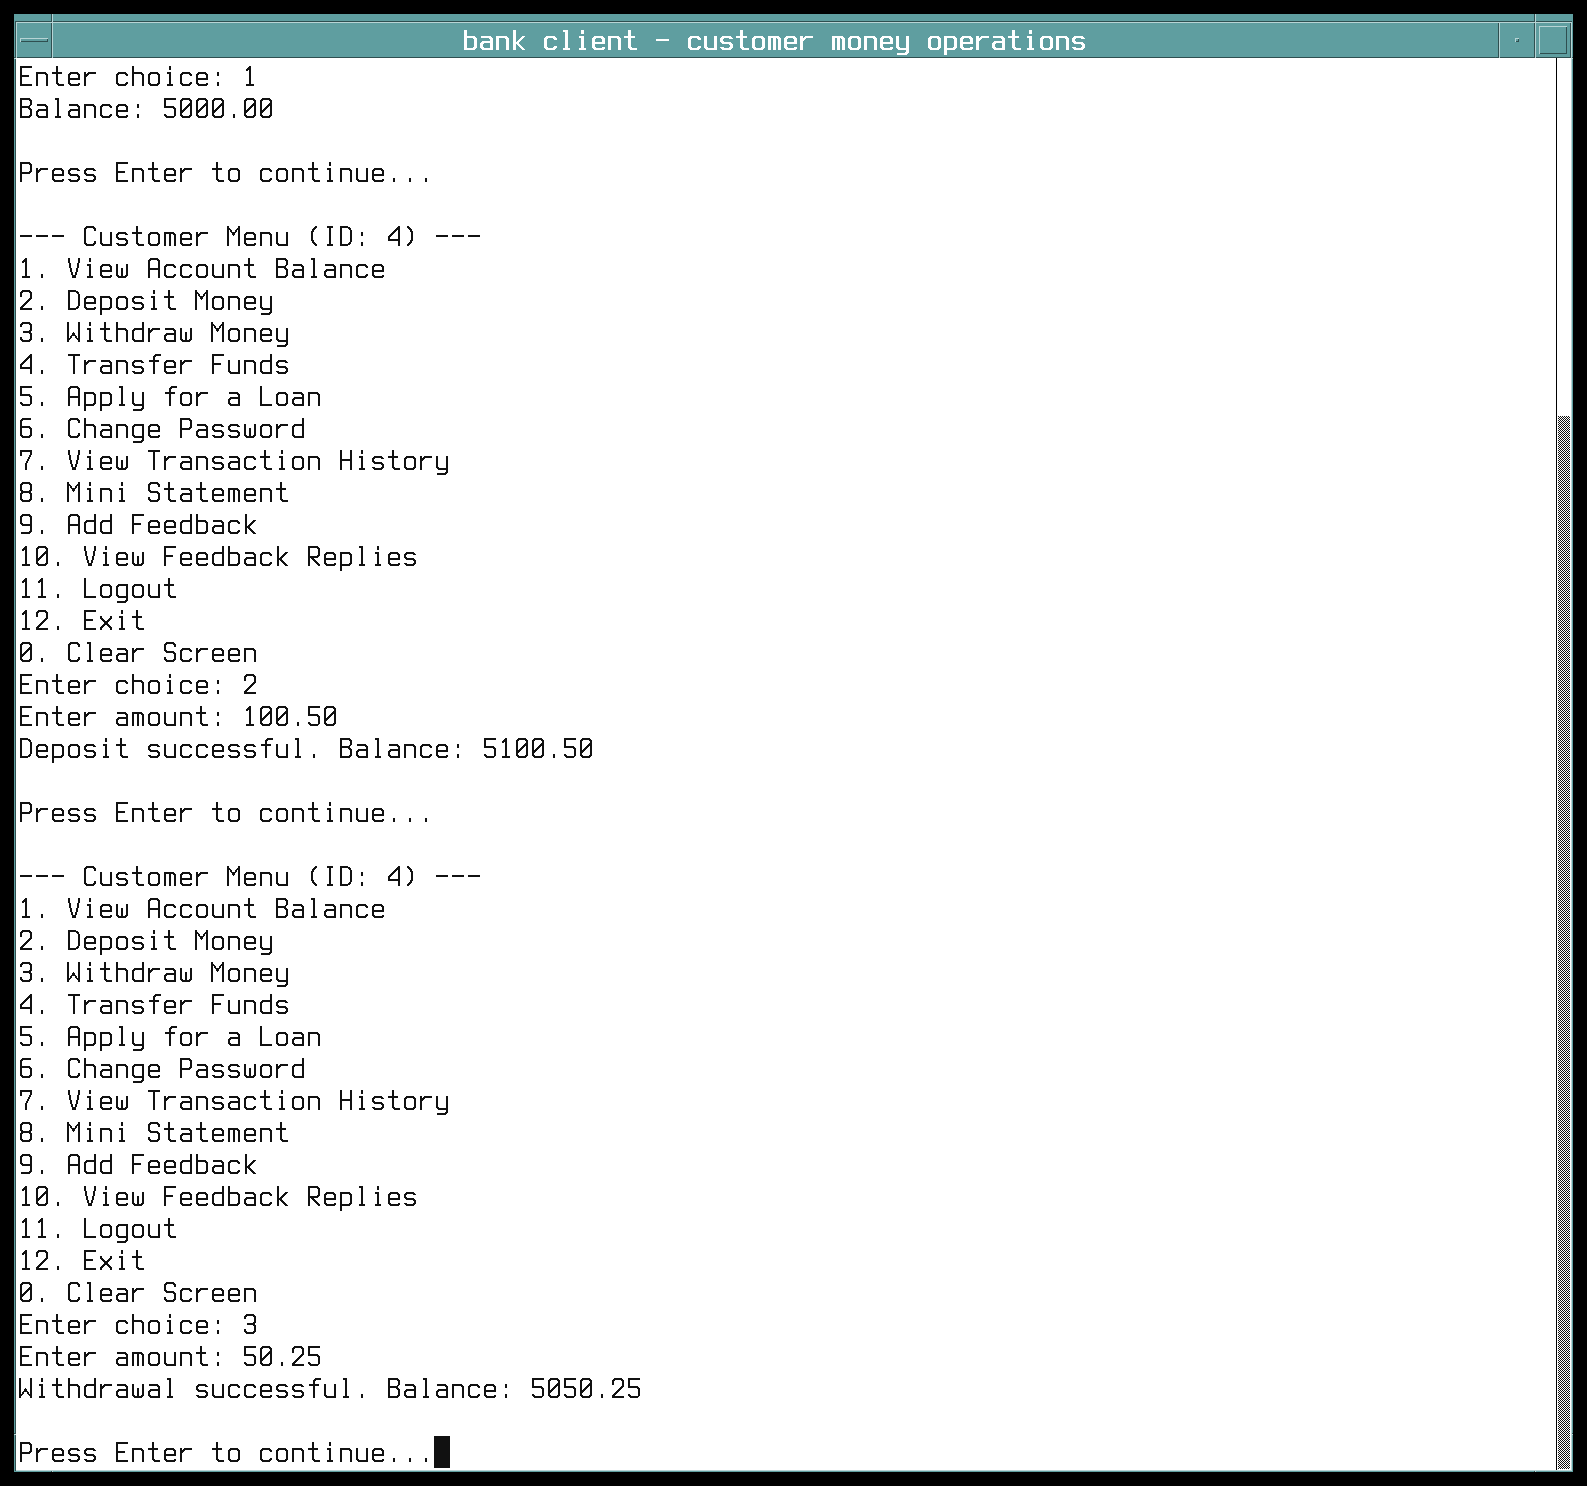
\includegraphics[width=0.64\linewidth]{05_customer_money.png}
\caption{The customer checks the balance, deposits, and withdraws.}
  \label{fig:customer-money}
\end{figure}
\begin{figure}[H]
  \centering
  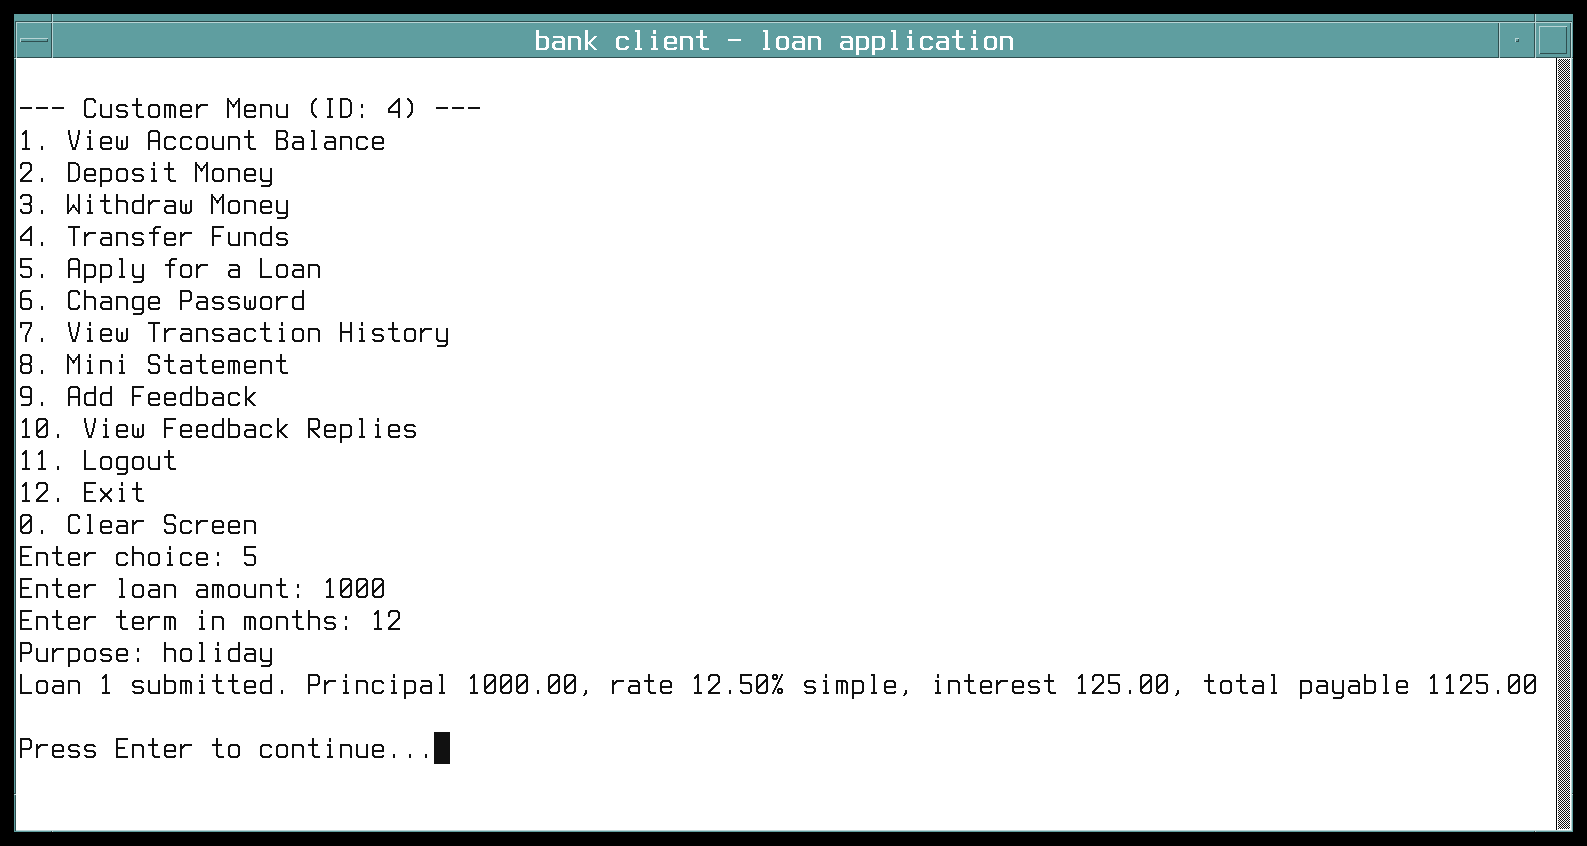
\includegraphics[width=0.64\linewidth]{08_loan_apply.png}
\caption{The customer applies for a loan with interest.}
  \label{fig:loan-apply}
\end{figure}
\begin{figure}[H]
  \centering
  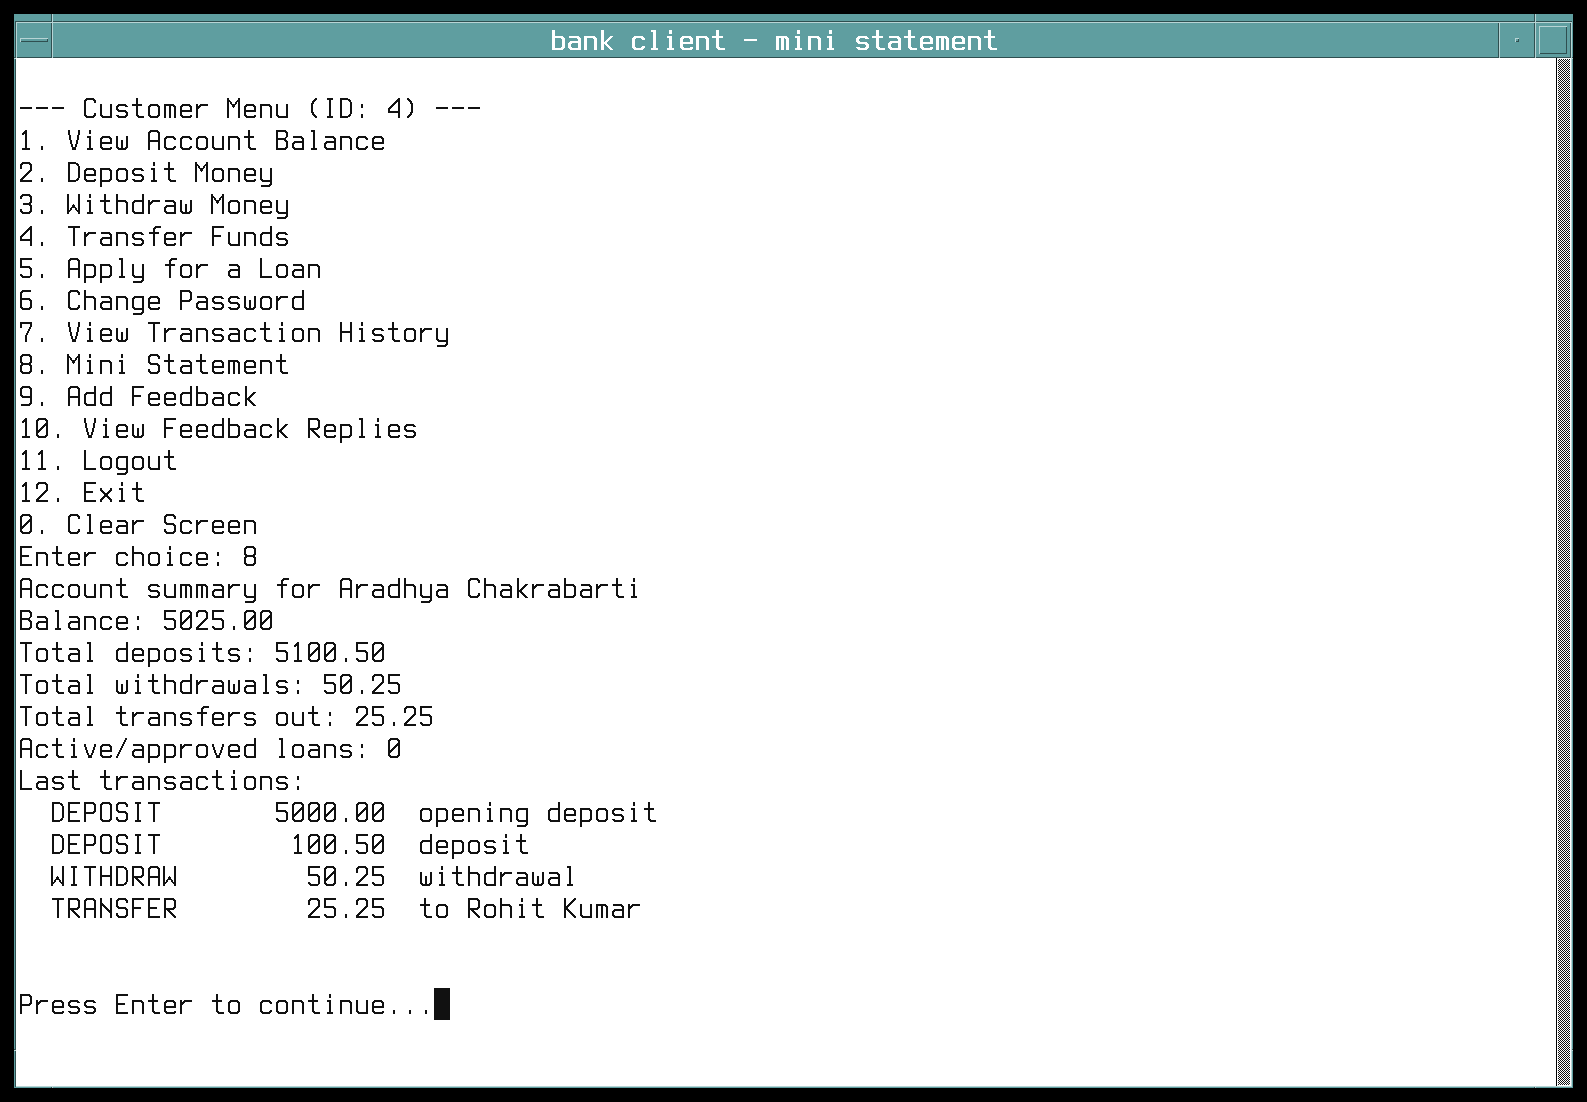
\includegraphics[width=0.64\linewidth]{07_mini_statement.png}
\caption{The customer views a mini statement.}
  \label{fig:mini-statement}
\end{figure}
\begin{figure}[H]
  \centering
  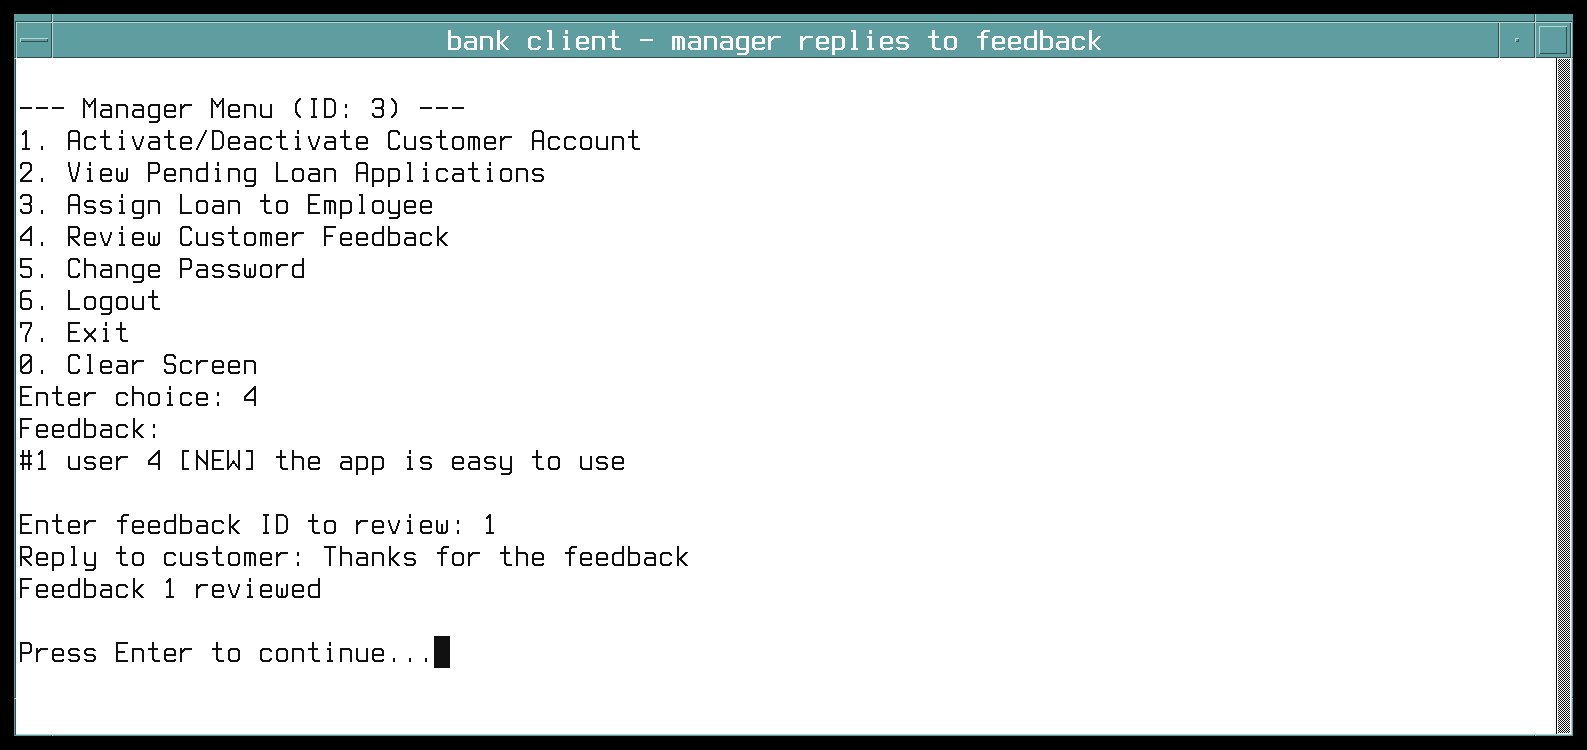
\includegraphics[width=0.64\linewidth]{12_manager_feedback.png}
\caption{The manager replies to feedback.}
  \label{fig:manager-feedback}
\end{figure}
\begin{figure}[H]
  \centering
  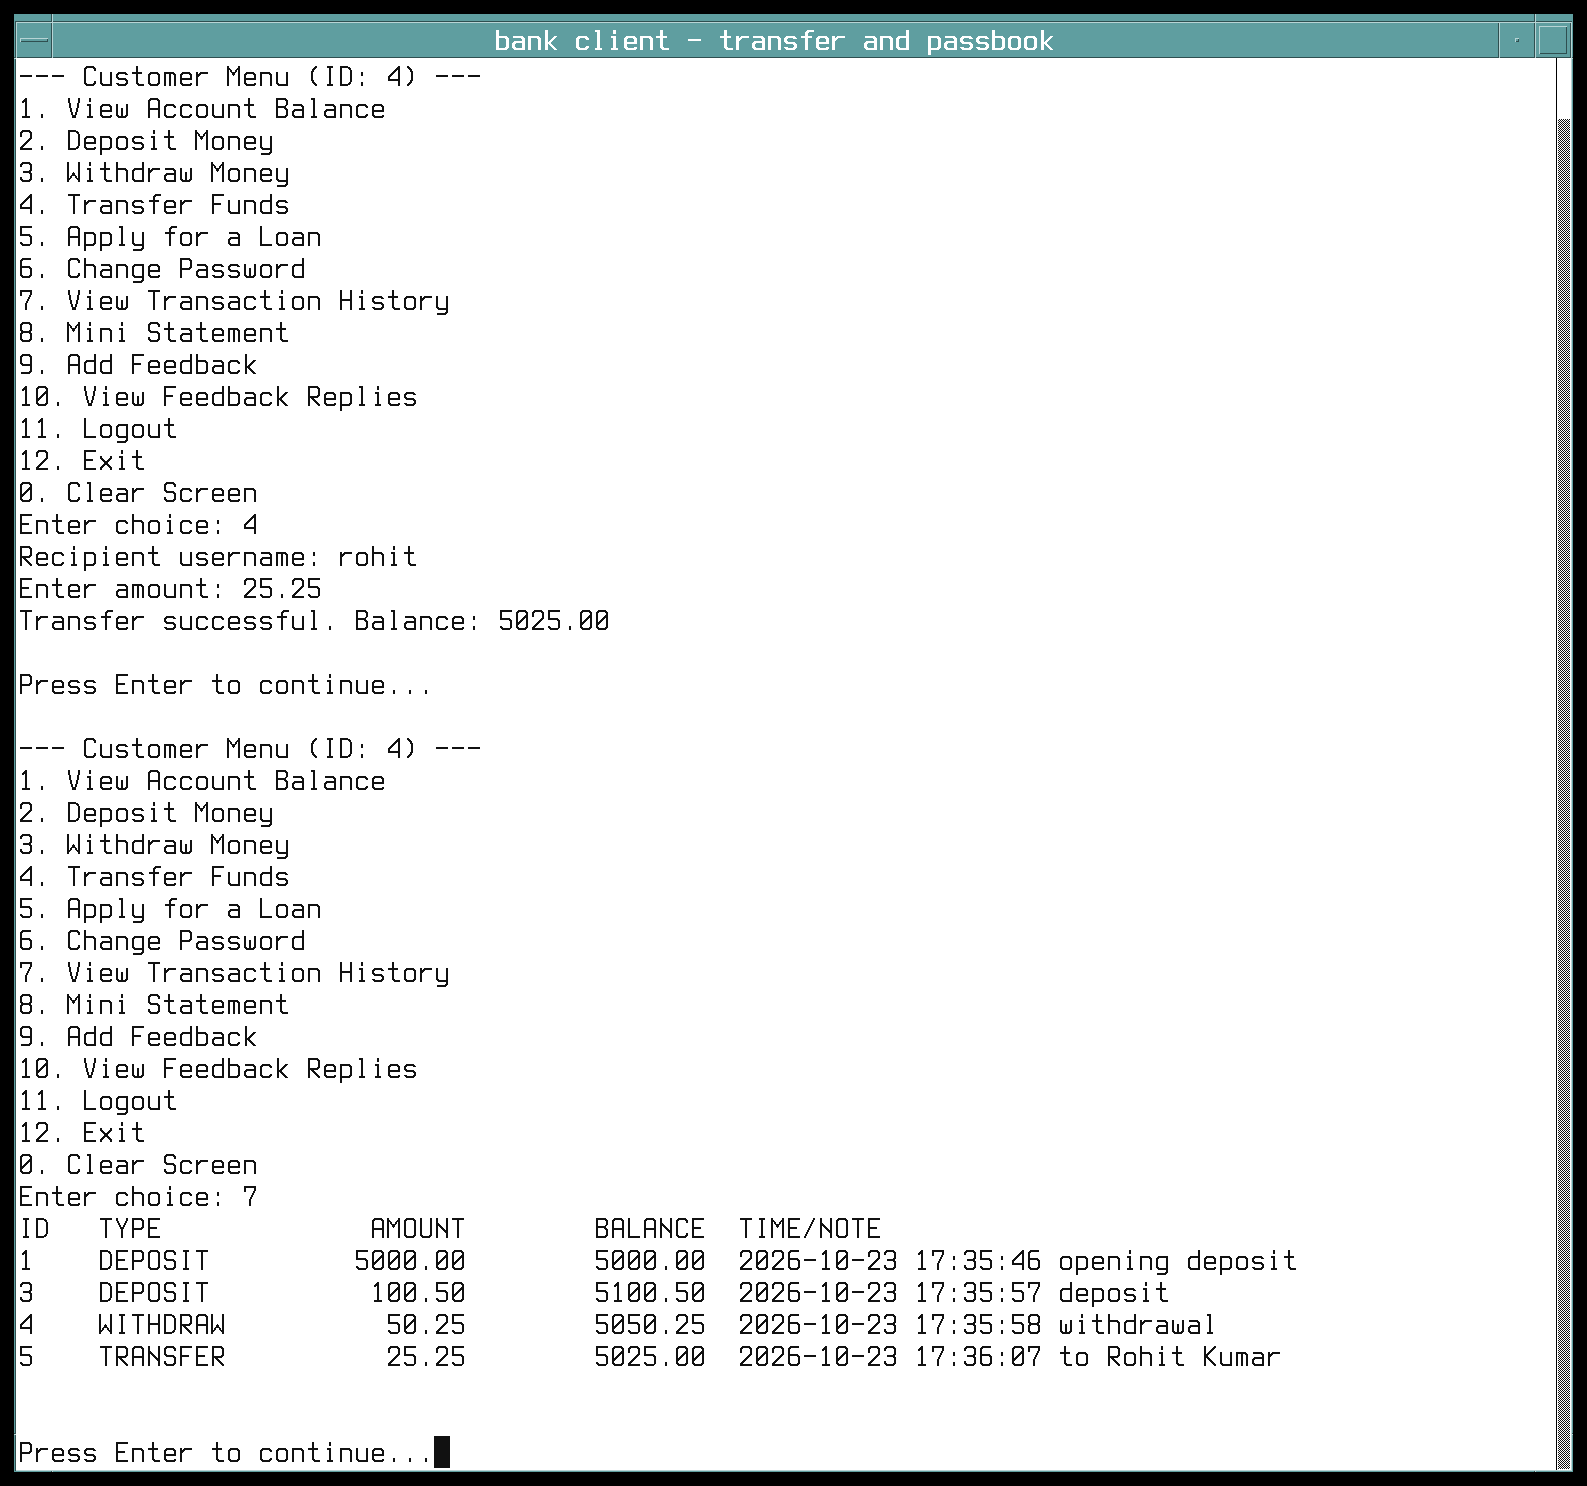
\includegraphics[width=0.64\linewidth]{06_customer_passbook.png}
\caption{The customer transfers funds and views the passbook.}
  \label{fig:customer-passbook}
\end{figure}
\begin{figure}[H]
  \centering
  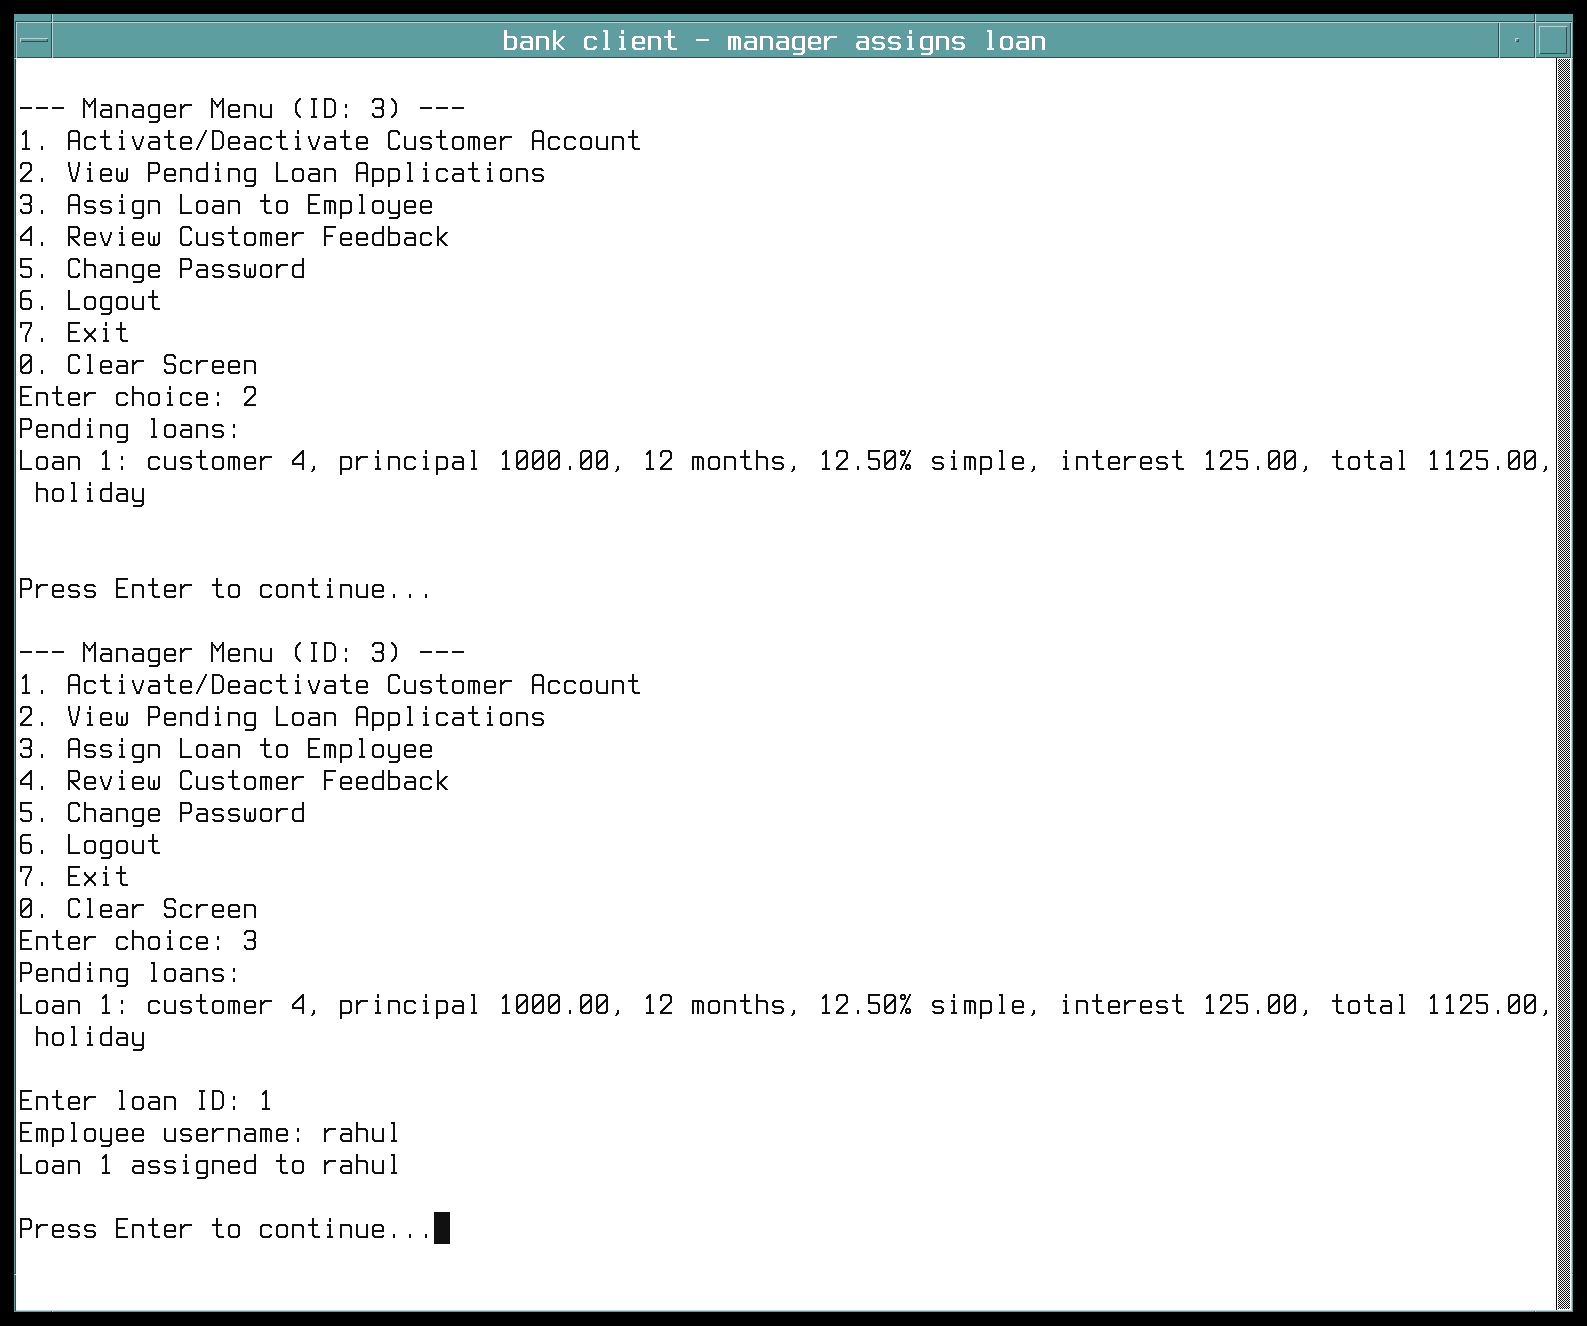
\includegraphics[width=0.64\linewidth]{09_manager_assign.png}
\caption{The manager assigns a pending loan.}
  \label{fig:manager-assign}
\end{figure}
\begin{figure}[H]
  \centering
  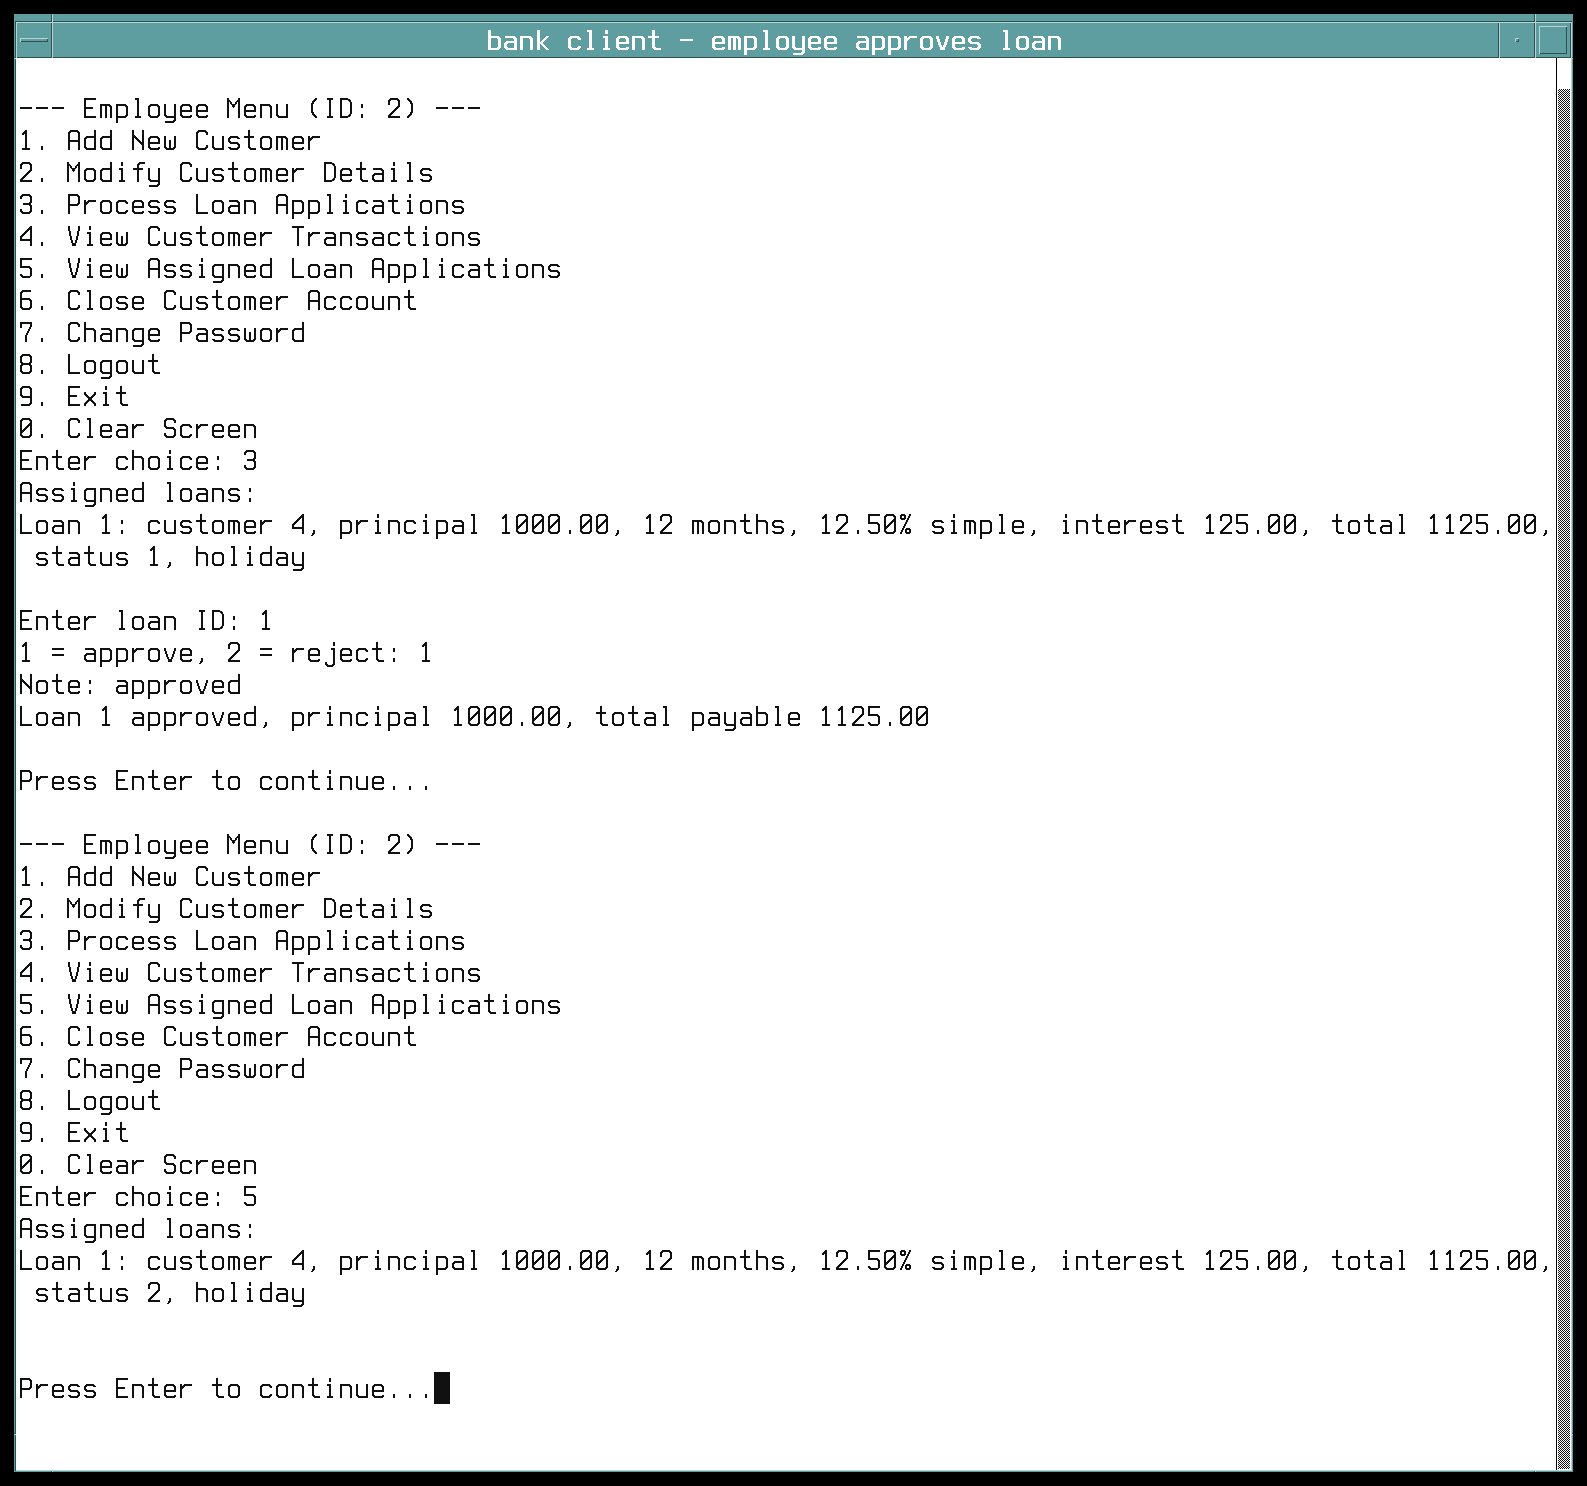
\includegraphics[width=0.64\linewidth]{10_employee_loan.png}
\caption{The employee approves the loan with the stored total payable.}
  \label{fig:employee-loan}
\end{figure}
\begin{figure}[H]
  \centering
  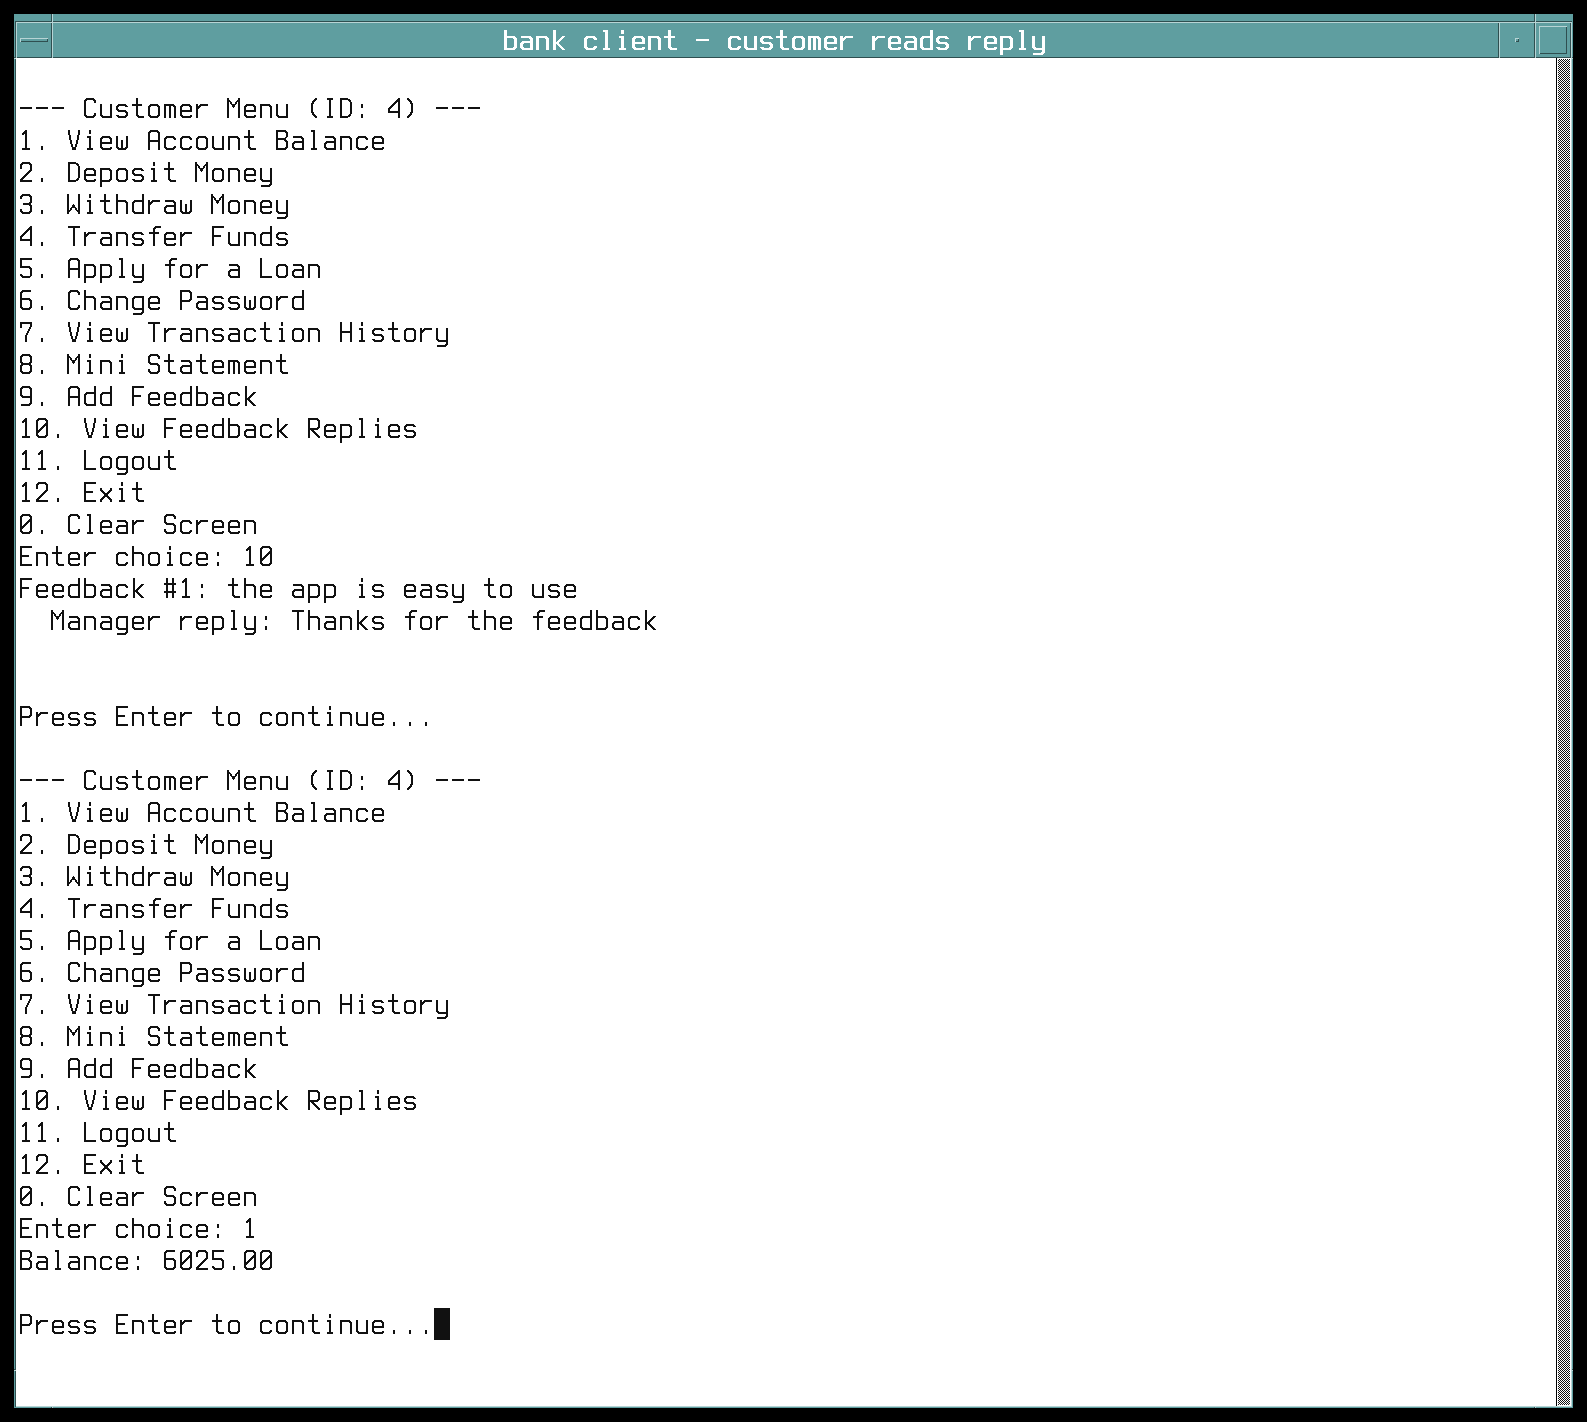
\includegraphics[width=0.64\linewidth]{13_customer_reply.png}
\caption{The customer reads the manager's reply.}
  \label{fig:customer-reply}
\end{figure}
\begin{figure}[H]
  \centering
  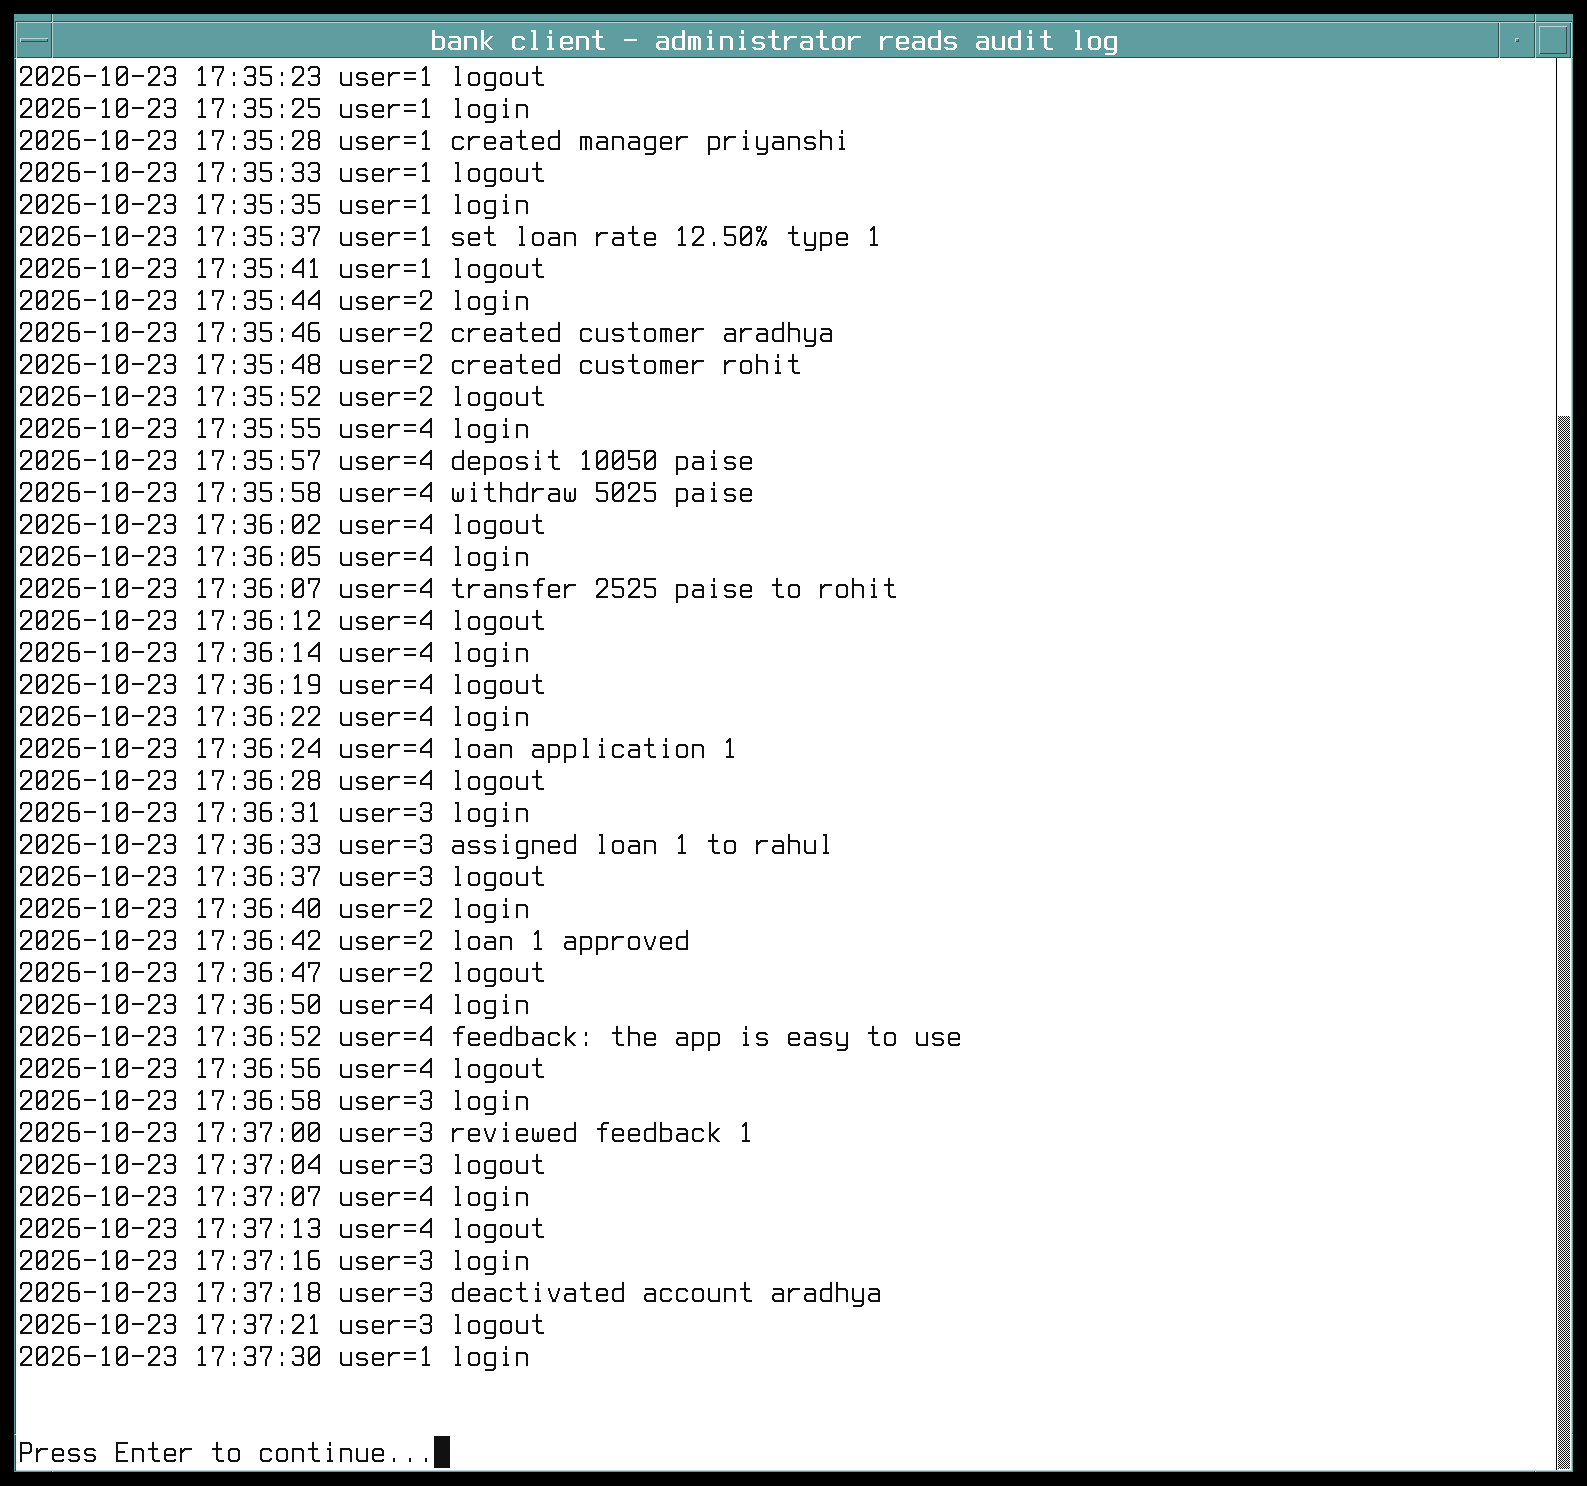
\includegraphics[width=0.64\linewidth]{16_admin_log.png}
\caption{The administrator reads the timestamped audit log.}
  \label{fig:admin-log}
\end{figure}
\subsection{Extras}

Three extra features were implemented.

\begin{itemize}
\item The mini statement (menu item 8) calls \texttt{do\_mini} and shows the balance, deposit, withdrawal, and transfer totals, the pending/approved loan count, and the last five transactions.
\item The feedback reply (manager item 4, customer item 10) stores a reply with \texttt{do\_review\_feedback} and reads it with \texttt{do\_my\_feedback}.
\item The loan interest policy (administrator item 6, customer item 5) stores one bank-wide rate and method. \texttt{do\_apply\_loan} copies the policy into each new loan, and existing loans keep their original policy.
\end{itemize}

\end{document}
